\documentclass[letter,12pt]{article}
\usepackage[letterpaper,right=1.25in,left=1.25in,top=1in,bottom=1in]{geometry}
\usepackage{setspace}

\usepackage[utf8]{inputenc}   % allows input of special characters from keyboard (input encoding)
\usepackage[T1]{fontenc}      % what fonts to use when printing characters       (output encoding)
\usepackage{amsmath}          % facilitates writing math formulas and improves the typographical quality of their output
\usepackage[hyphens]{url}     % adds line breaks to long urls
\renewcommand{\UrlFont}{\ttfamily\small} % shrinks url font 1 step down
\usepackage[pdftex]{graphicx} % enhanced support for graphics
\usepackage{tikz}             % Easier syntax to draw pgf files (invokes pgf automatically)
\usetikzlibrary{arrows}

\usepackage{mathptmx}           % set font type to Times
\usepackage[scaled=.90]{helvet} % set font type to Times (Helvetica for some special characters)
\usepackage{courier}            % set font type to Times (Courier for other special characters)

% \usepackage[longnamesfirst, sort]{natbib}\bibpunct[]{(}{)}{,}{a}{}{;} % handles biblio and references 
\usepackage[sort]{natbib}\bibpunct[]{(}{)}{,}{a}{}{;} % handles biblio and references 

\usepackage{rotating}         % sideway tables and figures that take a full page
\usepackage{caption}          % allows multipage figures and tables with same caption (\ContinuedFloat)

\usepackage{dcolumn}          % needed for apsrtable and stargazer tables from R to compile
\usepackage{arydshln}         % dashed lines in tables (hdashline, cdashline{3-4}, 
                              %see http://tex.stackexchange.com/questions/20140/can-a-table-include-a-horizontal-dashed-line)
                              % must be loaded AFTER dcolumn, 
                              %see http://tex.stackexchange.com/questions/12672/which-tabular-packages-do-which-tasks-and-which-packages-conflict

\usepackage{amssymb}          % has nicer empty set \varnothing, among much much more

%% %% FOR SPANISH FORMATTING (HYPHENATION ETC.)
%% \usepackage[spanish]{babel}
%% \addto\captionsspanish{\renewcommand{\figurename}{Diagrama}} % cambia Figura por Diagrama
%% \decimalpoint  % disable spanish's default comma decimal separator

\usepackage[longnamesfirst, sort]{natbib}\bibpunct[]{(}{)}{,}{a}{}{;} % handles biblio and references 
%% \AtBeginDocument{\renewcommand\harvardand{y}} % change 'author and author' by Spanish 'author y author'

\newcommand{\mc}{\multicolumn}

%% TO ADD NOTES IN TEXT, PUT % BEFORE THE ONE YOU WANT DISBALED
%\usepackage[disable]{todonotes}                            % notes not showed
\usepackage[colorinlistoftodos, textsize=small]{todonotes} % show notes
\newcommand{\eric}[1]{\todo[color=red!15, inline]{\textbf{Eric:} #1}}

% Format epigraph
\usepackage{epigraph}
\setlength\epigraphwidth{.8\textwidth}
\setlength\epigraphrule{0pt} % no rule

% multicolumns in appendix
\usepackage{multicol}

% change text color
\usepackage{xcolor}

% for code blocks
\usepackage{listings}

\setcitestyle{citesep={;}}

\usepackage{hyperref}

\usepackage{bigfoot}  %% allows the use of \verb command within footnotes

\begin{document}

\title{Antidote to the incumbency curse: \\ Mexico's reelection reform and municipal races 1997--2025\thanks{I am grateful to Francisco Garfias, Susan Stokes, and to participants at Tec de Monterrey's 4th Political Science Conference for suggestions on a preliminary version of the paper; to Gabino Martínez Díaz and Rodrigo Santibáñez Razo for research assistance; and for the generous support of the Asociación Mexicana de Cultura A.C. The author bears full responsibility for errors and limitations in the study.}}
\author{Eric Magar  \\ ITAM \\ \url{emagar@itam.mx}}
\date{\today}
\maketitle

% \begin{center} \textbf{$\rightarrow$~~Preliminary draft~~$\leftarrow$} \\ (please inquire for new version)  \end{center}

\begin{abstract}
\noindent Recent research uncovers systematic evidence of an incumbency curse in Mexican elections. The pattern resembles those found in other middle income democracies. A study of marginal municipal races between 1997 and 2010 revealed a discontinuity in the likelihood of winning the next election, estimating a .20 drop in the probability of reelecting in time t+1 the party that barely won in time t relative to the party that barely lost. This paper replicates the analysis by extending the data coverage to the following decade, when Mexico removed single-term limits for municipal governments. I find that the incumbency curse holds for races with an open seat. But when the incumbent mayor was on the ballot, the discontinuity is systematically reversed for every party. An incumbent mayor with static ambition therefore shields municipal parties from highly likely defeat.
\end{abstract}

%% Comentarios Susan Stokes: 27feb2026
%% - elaborar el proceso e historia del cambio institucional. La duración 12 años del régimen reeleccionista la leyó como one-shot.
%%   - EMM en esta misma línea, que sean reformas federales abona por la naturaleza exógena del cambio.
%% - Su lectura: disadvantage for the incumbent puzzling from US perspective --- elaborar esto.
%% - Libro de Luis Schiumerini sobre incumbency en LA
%% - Develop expectations, suggested effects of the scope of the office and responsibility should drive curse or advantage
%%   - EMM my take si pudiera separar algunos que se retiraron vs algunos pushed put, podría contener el efecto de selección.
%% - Su lectura: por selection bias, podría estar subestimando el efecto de la reforma (EMM no al revés?)
  
\newpage 

\onehalfspacing

\section{Introduction}

\noindent When a party takes over the reins of government, should its future electoral fortunes be expected to improve? Or, paradoxically, could they systematically worsen?

The emblematic and best-studied case, that of the U.S. Congress, points toward a substantial improvement in electoral fortunes. The incumbency advantage is such that it discourages the most serious challengers, who prefer to wait for better opportunities, resulting in comfortable victory margins for the incumbent and reelection rates exceeding 90 percent election after election.\footnote{\citet{erikson1971incumbency, mayhew1974vanishingMg, jacobson.1987.runningScared, cox.katz.1996, ansolabehere.snyder.IncAdv2002, gelman.king.1991incumbency}.} After 1955, Republicans had to wait almost the remainder of the twentieth century to wrest control of the House of Representatives from the Democrats.

I focus on municipal governments. Budget allocations, administrative appointments, and regulation through municipal ordinances are among the resources available to reward the electoral coalition from city hall. By channeling substantive benefits toward the groups that comprise it, these tools help sustain their loyalty to the party in future elections \citep{cox.mccubbins.1986, stokes.Argentina2005, diaz-estevez-magaloni-Poverty-book.2016}. However, it is also possible that these groups may have forged relationships not with the party itself but with one of its factions or cliques, and that such relationships may even be personal in nature \citep{cain.etal.1987}. In such cases, any shift in the balance among factions could cast doubt on their future loyalty to the party.

\citet{lucardi.rosas.Incumbency.2016} examined this question for Mexico, inspired by evidence from Brazil, India, Romania, and Zambia. In all these cases, social science research documents a systematic \emph{decline} in the probability of future victories for the governing party,\footnote{\citet{brambor.ceneviva.BrasilReeleccionMunic.2012, klasnja.titiunik.IncumbCurse.2023, uppal.IncumbencyIndia.2009}.} particularly at the sub-national level. Their analysis of municipal elections between 1997 and 2010 confirmed that Mexico follows the same pattern: governing today comes at the expense of winning again tomorrow.

This article presents preliminary results, incorporating a dimension absent from the original study: the possibility that the sitting mayor seeks reelection. Extending the Lucardi--Rosas model to the period following the adoption of this institution in Mexico reveals that the incumbency curse is conditioned by the retirement of the outgoing mayor. The curse appears to vanish for all major parties, when the incumbent mayor exhibits what \citet{schlesinger.1966} calls static ambition, that is, the desire to seek consecutive reelection to the same office. The argument unfolds as follows. The second section discusses the 2018 reelection reform and its recent counterreform. I then introduce marginal elections, the device exploited by the research design to measure the effect of the reform. The fourth section specifies a model that replicates Lucardi--Rosas while controlling for consecutive municipal reelection. After that \ldots

\eric{Revisar esto \citet{schiumerini.Incumbency2025, novaes.schiumerini.Commodity2022}.}

\section{Electoral reform} 

To everyone's surprise, electoral reformers in the middle of last decade eliminated the long-standing constitutional ban on consecutive reelection for municipal presidents and council members \citep{magar.el.dataset.2026}. Beginning in 2018, each state could decide whether to allow municipal authorities to seek consecutive reelection for one additional term only. With the exception of Hidalgo and Veracruz, all states allowed it, although at different times, as reported in Table \ref{T:reel}. Twenty-three states kicked-off reelection in 2018, removing single-term limits for a total of 1,382 municipal presidents whose terms ended that year. Three states did so in 2019, two in 2021, and the last two in 2024.

%% Year the reform kicked in. Column N reports the number of units electing municipal authorities per cycle (i.e., excluding /usos y costumbres/ municipalities). 
%% |    | edo |   yr |        N |
%% |----+-----+------+----------|
%% |  1 | ags | 2019 |       11 |
%% |  2 | bc  | 2019 |     5--7 |
%% |  3 | bcs | 2018 |        5 |
%% |  4 | cam | 2018 |       13 |
%% |  5 | coa | 2018 |       38 |
%% |  6 | col | 2018 |       10 |
%% |  7 | cps | 2018 | 124--125 |
%% |  8 | cua | 2018 |       67 |
%% |  9 | df  | 2021 |       16 |
%% | 10 | dgo | 2019 |       39 |
%% | 11 | gua | 2018 |       46 |
%% | 12 | gue | 2018 |   80--83 |
%% | 13 | hgo |    0 |       84 |
%% | 14 | jal | 2018 |      125 |
%% | 15 | mex | 2018 |      125 |
%% | 16 | mic | 2018 |      112 |
%% | 17 | mor | 2018 |       33 |
%% | 18 | nay | 2024 |       20 |
%% | 19 | nl  | 2018 |       51 |
%% | 20 | oax | 2018 |      152 |
%% | 21 | pue | 2021 |      217 |
%% | 22 | que | 2018 |       18 |
%% | 23 | qui | 2018 |       11 |
%% | 24 | san | 2018 |       58 |
%% | 25 | sin | 2018 |   18--20 |
%% | 26 | son | 2018 |       72 |
%% | 27 | tab | 2018 |       17 |
%% | 28 | tam | 2018 |       43 |
%% | 29 | tla | 2024 |       60 |
%% | 30 | ver |    0 |      212 |
%% | 31 | yuc | 2018 |      106 |
%% | 32 | zac | 2018 |       58 |

\begin{table}
  \centering
  \begin{tabular}{cccc}
    Kick-off        &   $N$      &                                           & $N$ municipalities \\ [-0.4ex]
    year            &  states    &  States                                   & per cycle  \\ \\ [-1.8ex] \hline \\ [-1.8ex]
    %Banderazo inicial  & $N$ estados & Estados    & $N$ municipios por ciclo \\ \hline
    2018            &          23 & All others                               & 1,382--1,388 \\
    2019            &           3 & Aguascalientes, Baja California, Durango &     55--57 \\
    2021            &           2 & Mexico City, Puebla                      &        233 \\
    2024            &           2 & Nayarit, Tlaxcala                        &         80 \\
    No reform       &           2 & Hidalgo, Veracruz                        &        296 \\ \\ [-1.8ex] \hline
  \end{tabular}
  \caption{The municipal electoral reform. The kick-off indicates the first year incumbent municipal officers could run for reelection. The number of observations per cycle varies because new municipalities were created in the period. Source: \citet{magar.el.dataset.2026}.}\label{T:reel}
  %\caption{La reforma electoral reeleccionista municipal. El banderazo inicial es el año a partir del cual un ocupante pudo estar en la boleta en busca de la reelección. El total de observaciones por ciclo es variable porque se crearon varios municipios nuevos en el periodo. Fuente: \citet{magar.el.dataset.2026}.}\label{T:reel}
\end{table}

Reformers never fully embraced the institution of reelection. For one thing, the move from single- to two-term limits was the mildest of feasible changes. And the new regime was lacking robustness: counter-reformers recently succeeded in backtracking, reinstating the constitutional consecutive reelection ban starting in the 2030 races.\footnote{A third aspect indicating hesitation was the reform's requirement that incumbents be renominated by the same party with which they won office, unless the party switch took place in the first half of the term. Formally, the party thus retained the ability to veto an ambitious mayor. In practice, however, many incumbent mayors in the data ran reelection campaigns with parties or coalitions other than the original. In all likelihood, the absence of an official record of party switchers and their timing among municipal officers (something that is routinely recorded by any assembly's steering board), rendered this requirement quite inoperable in municipal races. In practice, the requirement was constrained to legislative reelection only.} Six consecutive years in office, up from three, hardly qualifies as a distant time horizon, yet the short-lived regime (2018--2029) offers a unique opportunity to study how consequencial the adoption and removal of reelection was for local politics. Did the perspective of returning to office incentivize ambitious municipal officers to invest substantially in maintaining their electoral base alive and mobilized?  

\citet{motolinia-reel-book2026} is the most ambitious study of this brief Mexican interlude. True to a prolific literature initiated by \citet{mayhew.1974},\footnote{See \citet{jacobson.1987.runningScared,jacobson.1997,carey.etal.termLim.2000,carey.1996,cox.mccubbins.1993,shepsle.weingast.1994,kerevelPork2015,lucardi.micozzi.Career-argentina.2016,botero.renno-Career-reelec-br-col2007,morgenstern.nacif.2002,jacobson.kernell.1983}.} the inquiry focuses on legislative reelection only, examining the case of Mexico's state assemblies. The sub-national approach allows her to exploit the staggered kick-off dates to refine the empirical strategy. The study compiled and analyzed a monumental volume of evidence on state deputies (more than half a million assembly floor speeches, around ten thousand roll-call votes, committee assignments, as well as constituency service spending reports from thousands of members, and much more). Compared with other deputies, those who sought consecutive reelection doubled their probability of serving on committees with jurisdiction over particularistic policy (\emph{pork}); made 2 percent more references to district-oriented \emph{pork}-type projects in floor speeches; and reported constituency service budgets 15 percent larger. By contrast, metrics of party unity revealed no differences.

The effects Motolinia detects are systematic. As her theory of cross-cutting incentives predicts, they are notably small too. Party leaders' tight control of access to the ballot and the bulk of campaign resources leave little wiggle room for lawmakers to cultivate a personal, district-tailored style of campaigning. Perhaps there was not enough time for the institutional changes to mature. Or maybe the reform simply had no meaningful effects. Counter-reformers removed the chance to learn much more about this.

This article examines municipal \emph{presidents} in the same period. Unlike legislators, local executives spend continuously. At their disposal are relatively small budgets \citep{diaz.cayeros.2006}.\footnote{Most income in most municipalities comes through federal revenue sharing and earmarked federal investments. But municipal governments also have some authority to collect taxes \citep{magar.el.dataset.2026}, so, in principle, can loosen a hard budget by raising revenue.} But combined with their modest regulatory authority, municipal officers have capacity to create winners and losers among municipal dwellers. Deciding who gets appointments in the palacio municipal administration and allocating services to sub-contractors are key resources in spoils systems. Which, in turn, could be used to cultivate a personal vote \citep{cain.etal.1987,carey.shugart.1995}. I will show that the effects of the reelection institution---which, at best, appear faint in the legislative branch---operated noticeably and systematically among Mexican municipal executives.

\section{Close elections and the incumbency curse}

The literature inspiring this study places the focus in close elections, races decided by a small vote margin \citep{mayhew1974vanishingMg,cox.1999}. Despite taking place in very different regions, dates, and circumstances, close elections share a feature making them comparable: the winner is decided by the goddess Fortune.

To see this, consider two campaigns arriving to election day evenly matched: their candidates inspire confidence among similarly sized groups of voters, hits and misses in the campaign trail offset each other, they command comparable mobilization muscles, and so forth. When votes are counted, the anticipated outcome is a tie. Which is broken by fortuitous events: that food poisoning preventing wedding attendees from making it to the polls, the polling station unexpectedly voided due to irregularities, or voters confused by the ballot design.\footnote{A memorable case was Palm Beach County, Florida, in the 2000 presidential election (see \citet{nyt-cohn-palmbeach.2024}). The ballot was poorly designed, making a distracted or Gore voter an easy victim of inadvertently casting a vote for the third candidate, Buchanan. It may well have cost Gore the presidency. In Mexico, partial coalitions create room for asymmetric errors of the same nature: voters who, unintentionally, void their vote by supporting the coalition in places where it was not present.}

The analysis of close municipalities approximates a controlled experiment. In the present case, it constitutes a quasi-experimental design to measure the effect of governing or being in opposition—treated as a randomized treatment—on the party’s future electoral fortunes. If the probability of winning close municipalities is systematically higher where the party previously lost than where it previously won, this would reveal a \emph{municipal incumbency disadvantage}.

Lucardi and Rosas uncover such a pattern for Mexican municipal parties, without exception. Table \ref{F:luro-res} portrays it (it is a snapshot of their Fig. 1, p. 70). The X-axis measures mg$_t$, the percentage margin separating the winner from the main challenger in the municipal election of year $t$. Cases where the party was the main challenger display negative margins; cases where it won show positive margins. The Y-axis measures $p_{t+1}$, the probability that the party wins the next election. One party at a time, they classify municipal elections in the 1997--2010 period into three groups: a) those the party barely won,\footnote{In their analysis, Lucardi and Rosas consider a $\pm 15\%$ range as the selection criterion. Since \citet{mayhew1974vanishingMg}, it has been more common to consider elections decided by a single-digit vote margin, $\pm 10\%$, as close. I adopt that criterion here.} which appear on the right side of the diagrams, starting at the central vertical line; b) those it barely lost, which appear on the left side with negative margins; and c) all elections that were not close, which they discard from the analysis.

\begin{figure}
  \centering
  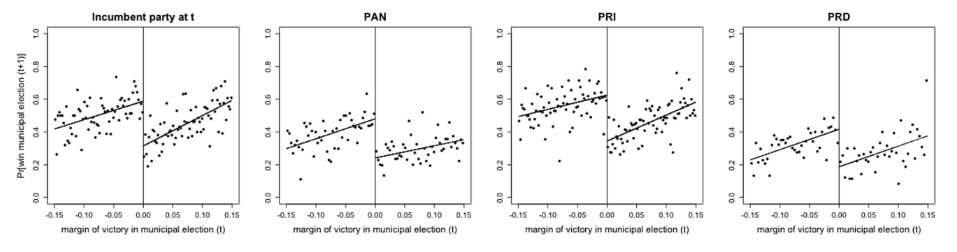
\includegraphics[width=\columnwidth]{../plots/luro-fig1.png}
  \caption{Resultados Lucardi--Rosas: la probabilidad de reelegir al partido municipal}\label{F:luro-res}
\end{figure}  

They estimate $p_{t+1}$, conditional on mg$_t$, separately for the left and right samples. The gap in the intercepts of the dashed regression lines stands out. The estimated probability of reelecting the PRD and the PAN in $t+1$ was on the order of .2 when they barely won in year $t$, but about .4 when they barely lost in year $t$. The gap for the PRI is even wider, with probabilities of .3 and .6, respectively.

A paradox of Mexican electoral democracy: as if a curse fell upon city hall, the three parties of the partidocracy era doubled their prospects of winning the next election simply by remaining in the opposition.

\section{A model with consecutive reelection}

Shortly after the period analyzed by Lucardi--Rosas, the reelection reform took place, with the potential to shake up municipal elections in Mexico. Beginning with the 2018 elections, the prohibition on the consecutive reelection of municipal authorities was progressively eliminated.

If, as suggested above, the obstacle faced by the municipal party has been persuading the electoral coalition that another term ``under new management'' would maintain the previous redistribution, then the reformers directly and squarely intervened in the problem. Because, through the personal vote \citep{cain.etal.1987}, the mayor’s renomination should mitigate that distrust. And perhaps bring an end to the incumbency curse.

% $I\kern-0.15em P(\text{gana}_{t+1})$

To evaluate this hypothesis, I replicate the Lucardi--Rosas model while controlling for static ambition. To analyze the probability $p_{t+1}$, I estimate the following regime-switching model:

\begin{equation}\label{E:model}
\begin{split}
\text{logit}\bigl(p_{t+1}\bigr) =~  & ~~~~~~~~~~~~~\text{neg}_t~ \times (\alpha_0 + \alpha_1 \text{inc}_{t+1} + \alpha_2 \text{mg}_t + \alpha_3 \text{inc}_{t+1} \times \text{mg}_t) \\
                                   & +~ (1 - \text{neg}_t) \times (\beta_0 + \beta_1 \text{inc}_{t+1} + \beta_2 \text{mg}_t + \beta_3 \text{inc}_{t+1} \times \text{mg}_t)  \\
 & +~ \text{error}_{t+1}
\end{split}
\end{equation}

\noindent where mg$_t$ is the independent variable already introduced. On the right-hand side it is accompanied by two dichotomous indicators and a random disturbance. The variable neg$_t$ takes the value one when $\text{mg}_t < 0$ and zero when $\text{mg}_t>0$. In the specification, $\text{neg}_t$ indicates the change in the estimation regime (the discontinuity): the $\beta$ parameters capture effects when the party entered government in $t$, while the $\alpha$ parameters capture effects when it remained out of office in that year.

% Al restringir los casos de estudio a las elecciones marginales solamente ($-.10 < \text{margen}_t < .10$), el cambio de régimen se interpreta como un tratamiento aleatorizado: un empate resuelto al azar.

And the indicator $\text{inc}_{t+1}$ takes the value one when the incumbent mayor runs for reelection in $t+1$, and zero otherwise. It allows for a shift in the intercept for elections with/without the incumbent on the ballot. Its multiplicative interaction with the margin in equation \ref{E:model} also estimates a possible change in slope.

\section{The data and their subsets}

\noindent I anticipate three obstacles to estimating the effect of the reform on the probability of reelection of the municipal party. One is associated with the self-selection of competitors, another with the collapse of the party system of the democratic transition, and the third with the ubiquity of electoral coalitions.

\subsection{Self-selection}

\begin{table}
  \centering
  %|        Año | Pre-banderazo | Alcalde contendió | Silla vacía | Term-limit | Total |      |
  %|       2018 |           227 |               508 |        1092 |          0 |       | 1600 |
  %|       2019 |             5 |                26 |          29 |          0 |       |   60 |
  %| 2018--2019 |           232 |               534 |        1121 |          0 |       | 1660 |
  %|       2021 |            80 |               605 |         735 |        268 |       | 1688 |
  %|       2022 |             0 |                17 |          27 |          9 |       |   53 |
  %| 2021--2022 |            80 |               622 |         762 |        277 |       | 1741 |
  %|       2024 |             0 |               777 |         606 |        321 |       | 1704 |
  %|       2025 |             0 |                16 |          18 |          5 |       |   39 |
  %| 2024--2025 |             0 |               793 |         624 |        326 |       | 1743 |
  \begin{tabular}{crrrrrrr}
               & \mc{3}{c}{Post-kick-off}&          &           &       &       \\ \\ [-1.8ex]\cline{2-4} \\ [-1.8ex]
               &      (1) &   (2) &  (3) &      (4) &       (5) & \mc{2}{c}{(6)}\\
               & Incum-   & Term  & Open & Pre-     & Non       &       &       \\ [-0.4ex]
    Years      & bent ran & limit & seat & kick-off & reformers & Total &  $N$  \\ [1ex] \hline \\ [-1.8ex]
    2018--2020 &       30 &     0 &   51 &       13 &         5 &   100 & 1,745 \\
    2021--2023 &       32 &    14 &   39 &        4 &        11 &   100 & 1,955 \\
    2024--2026 &       38 &    16 &   31 &        0 &        15 &   100 & 2,039 \\ 
    Total      &       34 &    11 &   39 &        5 &        10 &   100 & 5,739 \\
    %%            & Pre-          & Ocupante          & Silla       & Term       &       &      \\ [-0.4ex]
    %% Años       & banderazo     & contendió         & vacía       & limit      & Total &    N \\ [1ex] \hline \\ [-1.8ex]
    %% 2018--2019 &            14 &                32 &          54 &          0 &   100 & 1,660 \\
    %% 2021--2022 &             5 &                36 &          44 &         16 &   100 & 1,741 \\
    %% 2024--2025 &             0 &                45 &          36 &         19 &   100 & 1,743 \\ 
    %% Total      &             6 &                38 &          44 &         12 &   100 & 5,144 \\
    \\ [-2ex] \hline
  \end{tabular}
  \caption{Tickets with and without an incumbent municipal president running 2018--2025. Columns 2--5 distinguish the cases with no incumbent running. Sources: \citet{magar.el.dataset.2026}.}\label{T:incballot}
\end{table}

\noindent The first obstacle is that municipal presidents have some degree of agency in deciding whether to seek consecutive reelection or to refrain from doing so. Table \ref{T:incballot} shows that 38 percent of incumbents in the period ran for reelection. While this figure signals enthusiasm for the reform among municipal officeholders, it also reports that 44 percent did not run despite having the opportunity to do so. This self-selection should magnify the effect on the probability I seek to measure. To see this, imagine two types of mayors: those who anticipate an impossible reelection campaign, and those who expect a campaign without major difficulties. If these expectations were accurate and all incumbents ran, the first group would obtain noticeably less favorable results, and much higher defeat rates, than the second. This should also push them to withdraw with greater probability than the latter, thereby widening margins and reelection rates.

This phenomenon is problematic for anyone seeking an identification strategy for the causal effect of ending the prohibition (the treatment) \emph{without} this self-selection effect.\footnote{And it could be mitigated with empirical indicators---which I do not have---to distinguish voluntary withdrawals, of the kind just discussed, from those driven by reasons orthogonal to expectations, such as when a party successfully vetoes a mayor’s reelection ambitions.} By contrast, I am interested in measuring both together, because consecutive reelection is an institution designed precisely to allow those with advantages, those who have cultivated their electoral coalition, to in fact \emph{self-select} into running again. From the perspective of my argument, the first is simply not an obstacle: self-selection is something I seek to capture empirically.

%% \begin{table}
%%   \centering
%%   \begin{tabular}{r|lc|lc|}
%%                   & \mc{4}{c}{Tiene ambición estática}                 \\
%%                   & \mc{2}{c}{No}       &    \mc{2}{c}{Sí}             \\ \hline
%%     Renominado No & $a$ & se retira     & $b$ & lo retiran             \\ \cline{2-5}
%%                Sí & $c$ & $\varnothing$ & $d$ & compite de nuevo \\ \hline
%%   \end{tabular}
%% %%  \caption{Self-selection is confouded. The study cannot separate observations in cells $a$ and $b$, which presumably correlate with party performance.}\label{T:matrix}
%%   \caption{La auto-selección confundida. El estudio no puede distinguir observaciones en las celdas $a$ y $b$, que se correlacionan con desempe partidista.}\label{T:matrix}
%% \end{table}

%% La matriz de 2-por-2 del cuadro \ref{T:matrix} ilustra el primer obstáculo, cruzando el deseo de buscar la reelección consecutiva (la ambición estática de Schlesinger) con el éxito en ser renominado para contender. El cuadro supone que quienes no aspiran a reelegirse declinarían la nominación, si se las diera el partido---y la celda $c$ está vacía. (Podría no ser así, siempre es concebible que alguien te haga recapacitar cuando declinas... omito esta complicación.) Lo que sí contempla el cuadro es la posibilidad de que quien aspire a la reelección no consiga la nominación, lo que llamo `ser retirado' (celda $b$), distinto de `retirarte' (celda $a$). El obstáculo radica en que la evidencia no permite distinguir observaciones en las celdas $a$ y $b$.  

\subsection{The AMLO effect}

\begin{table}
  \centering
  \begin{tabular}{@{\extracolsep{5pt}}lrrrrrrrr}
    & &                        & \mc{4}{c}{2018--2025}  \\ \cline{4-7}
    & \mc{2}{c}{(1)} & \mc{2}{c}{(2)} & \mc{2}{c}{(3)} & \mc{2}{c}{(4)} \\
 & \mc{2}{c}{1997--2017} & \mc{2}{c}{Pre-kick-off} & \mc{2}{c}{Post-kick-off} & \mc{2}{c}{1997--2025} \\ \cline{2-3} \cline{4-5} \cline{6-7} \cline{8-9}
%% & \mc{2}{c}{1997--2017} & \mc{2}{c}{Pre-banderazo} & \mc{2}{c}{Post-banderazo} & \mc{2}{c}{1997--2025} \\ \cline{2-3} \cline{4-5} \cline{6-7} \cline{8-9}
 Partido    & opos. & ocup. & opos. & ocup. & opos. & ocup. & Total &     N \\ [1ex] \hline \\ [-1.8ex]
 Izquierda  & 35.0 & 38.7 & 1.6 & 1.5 & 11.7 & 11.5 & 100.0 & 3,896 \\
 PAN        & 32.1 & 32.9 & 1.4 & 1.3 & 15.1 & 17.2 & 100.0 & 5,623 \\
 PRI        & 39.6 & 35.1 & 0.9 & 1.0 & 12.0 & 11.3 & 100.0 & 7,868 \\ 
    \\ [-2ex] \hline
  \end{tabular}
  \caption{Three subsets of close elections in 1997--2025 used for the estimations. Before 2015, the left corresponds to the PRD; starting in 2018 it corresponds to Morena; and in the intervening years it refers to either of the two. Sources: \citet{magar.el.dataset.2026}.}\label{T:data}
%  \caption{Tres subconjuntos de elecciones marginales en 1997--2025 para las estimaciones. Antes de 2015, la izquierda es el PRD, desde 2018 es Morena, y entre esos años es cualquiera de ambos. Fuentes: \citet{magar.el.dataset.2026}.}\label{T:data}
\end{table}

\noindent The collapse of the party system, however, could complicate the measurement of the effect of the new institution, because the critical election of 2018 coincided with the first kick-off. Changes in performance could be attributed either to the end of the reelection ban, to the emergence of Morena—a party that realigned the Mexican electorate—or to both. As Motolinía does, I exploit the staggered timing of the kick-offs as leverage for disentangling these effects, analyzing different subsets of observations. Table \ref{T:data} summarizes them.

For all my estimations I select exclusively close municipal elections ($\pm10\%$) in the period of democratic elections beginning in 1997. Column (4) reports the number of observations for each party. I begin by estimating the models using the full set of elections from 1997--2025, which includes (and thus conflates) both the tripartite system of democratization and the Obradorista system that replaced it. The number of observations for the left, the PAN, and the PRI varies because I include those municipalities where, in the previous cycle, each party either narrowly won or narrowly finished in second place. The obstacle is particularly evident in the case of the left, since I had to select two parties: from 2018 onward this refers to Morena, before 2015 to the PRD, and between 2015 and 2017 to either of these two parties.\footnote{There are three observations between 2015 and 2017 in which the winner and the runner-up corresponded to Morena and the PRD. I removed these three observations from the sample. There were only three because the lack of coordination that Morena introduced into the electoral left beginning in 2015 often pushed both parties below the margin, granting artificial victories to the PRI.}

To attempt to circumvent this obstacle, I then estimate the models for the 2018--2025 period, the Obradorista party system. I analyze separately two mutually exclusive subsets of observations. The first corresponds to the states that, after AMLO’s critical election, had not yet given the starting signal for municipal reelection (column 2). These allow us to verify whether the Lucardi--Rosas patterns replicate, in the absence of the reelection institution, after AMLO’s election in 2018, which was concurrent with the municipal contests. The second subset corresponds to the states that had already adopted the reelection reform, where one would expect a possible change as a consequence of the new institution (column 3).

(Finally, the appendix also replicates the estimation for the 1997--2017 period (column 1), in order to corroborate that my study finds patterns identical to those of Lucardi--Rosas.)

\subsection{Coalitions}

\noindent The third obstacle arises from the frequent pre-electoral coalitions formed by parties. \citet{magar.el.dataset.2026} and \citet{spoon.pulido.PRI-PVEM2017} provide further detail. Proscribed during the classic PRI era, democratization made them common rather quickly. For the 2006--2008 cycle, for example, four out of five municipal elections featured one or more coalitions, and the proportion has remained similar to this day.

Originally these were coalitions between a major party (the PRI, PAN, or PRD) and one or more opportunistic minor parties (PVEM, PT, etc.), aimed at refreshing the vote and improving the major party’s chances of victory. But since 2010 anti-PRI coalitions between the PAN and the PRD became common. And after 2018, anti-Morena coalitions among the PAN, PRI, and PRD.

The difficulty for the analyst is one of attribution: to which of the coalition parties should victory or defeat be assigned? The selection of close municipal elections requires an indicator of the parties that finished in first and second place. It seems safe to award the victory to the major party when it coalitions only with minor parties. But doubts arise when coalitions involve more than one major party. Consider, for example, the municipality of Durango, which the PAN--PRD coalition won in 2016. In 2019 the PAN won on its own; in 2022 the PAN--PRI--PRD coalition prevailed; and in 2025 Toño Ochoa was reelected mayor but with a PAN--PRI coalition. A literal reading would indicate that the PRD won in 2016 and in 2022, and lost in the other years. If, instead, we incorporated knowledge of Durango’s party system, we would discount the PRD because it is a very minor party in the state. If we further incorporated the fact that Toño Ochoa has been a prominent PAN politician, we would probably also discount the PRI in the victories of 2022 and 2025.

Unfortunately, I do not have this information to conduct a systematic analysis of thousands of municipal elections. The estimates presented below take a literal reading of coalitions. In future iterations of the article I will use finer classification criteria (such as coalition agreements, the governor’s party, the historical vote share of parties in each municipality, etc.) to attempt to show that my findings are not the result of this particular coding of coalitions among major parties.

\section{Results}

\noindent I first present the patterns from the estimation using the full period before proceeding to a more fine-grained analysis. (For these initial models I used a Bayesian estimation with the MCMC method, and the diagrams use a sample from the posterior distribution—for the final version of the remaining models I will use this same methodology in parallel with the standard OLS estimation of the models.) As in Lucardi--Rosas, the incumbency curse appears in the brown portion of the diagrams for the left, the PAN, and the PRI, patterns analogous to those observed above. The brown portion corresponds to municipal elections where the incumbent does not run, and the gap in the intercepts is notable.

\begin{figure}
  \centering
  %% \begin{tabular}{ccc}
  %% 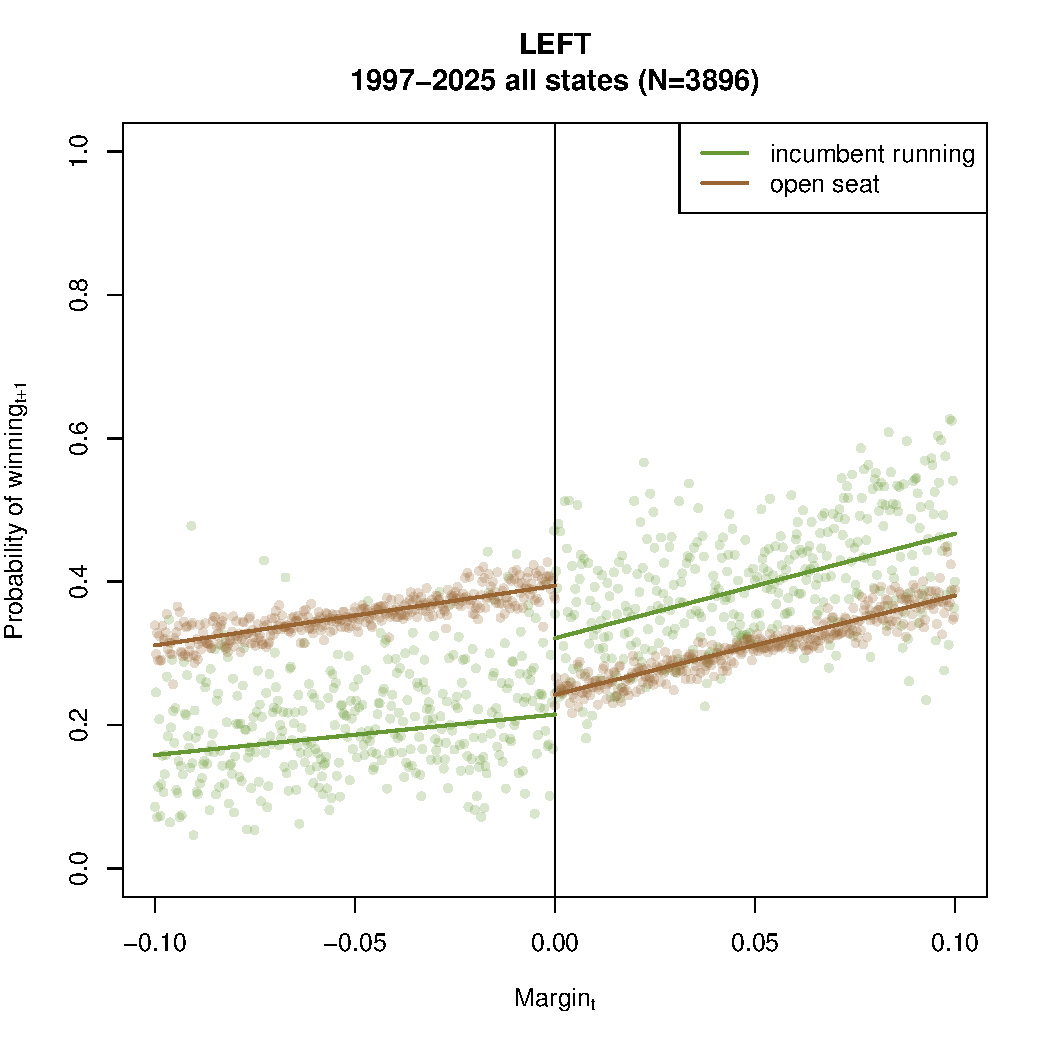
\includegraphics[width=.31\columnwidth]{../plots/left4ALLmcmc.pdf} &
  %% 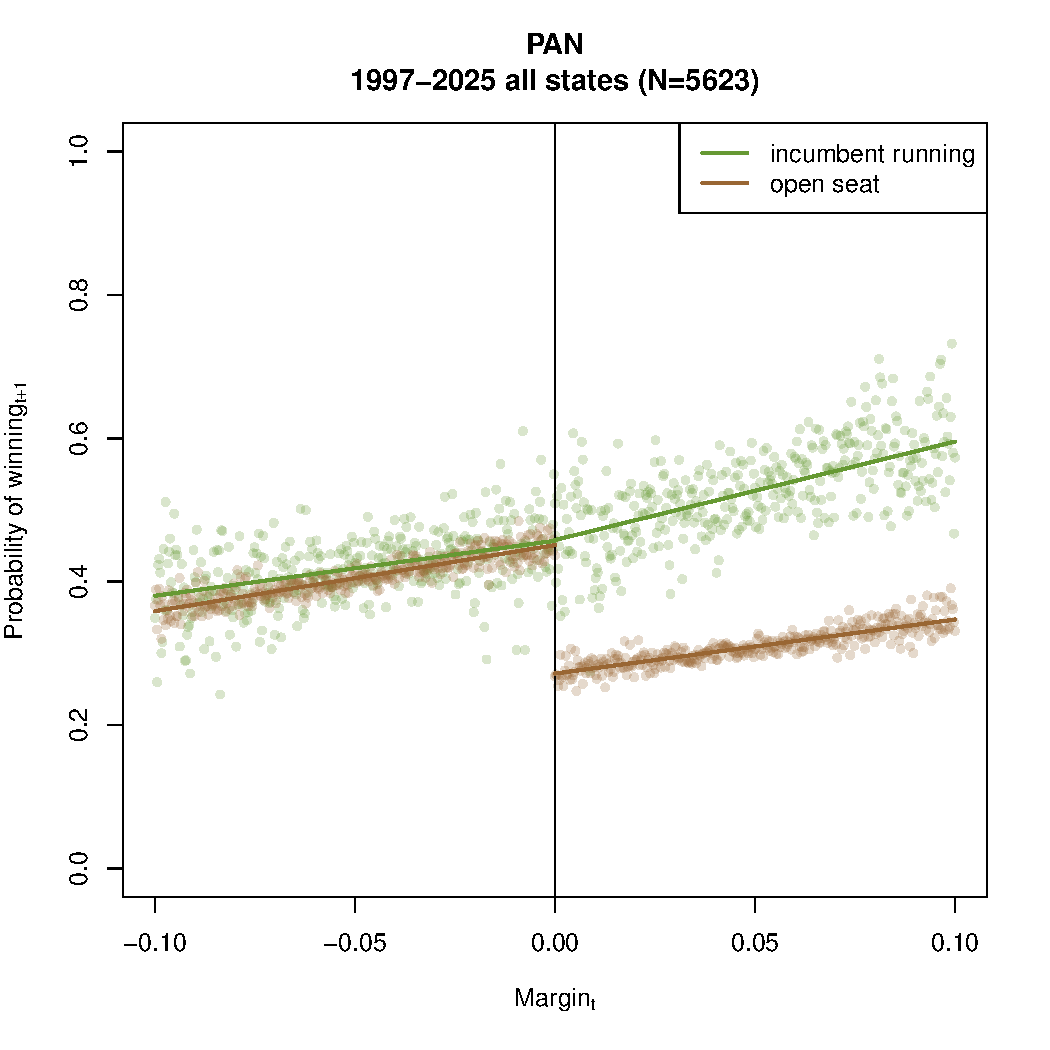
\includegraphics[width=.31\columnwidth]{../plots/pan4ALLmcmc.pdf} &
  %% 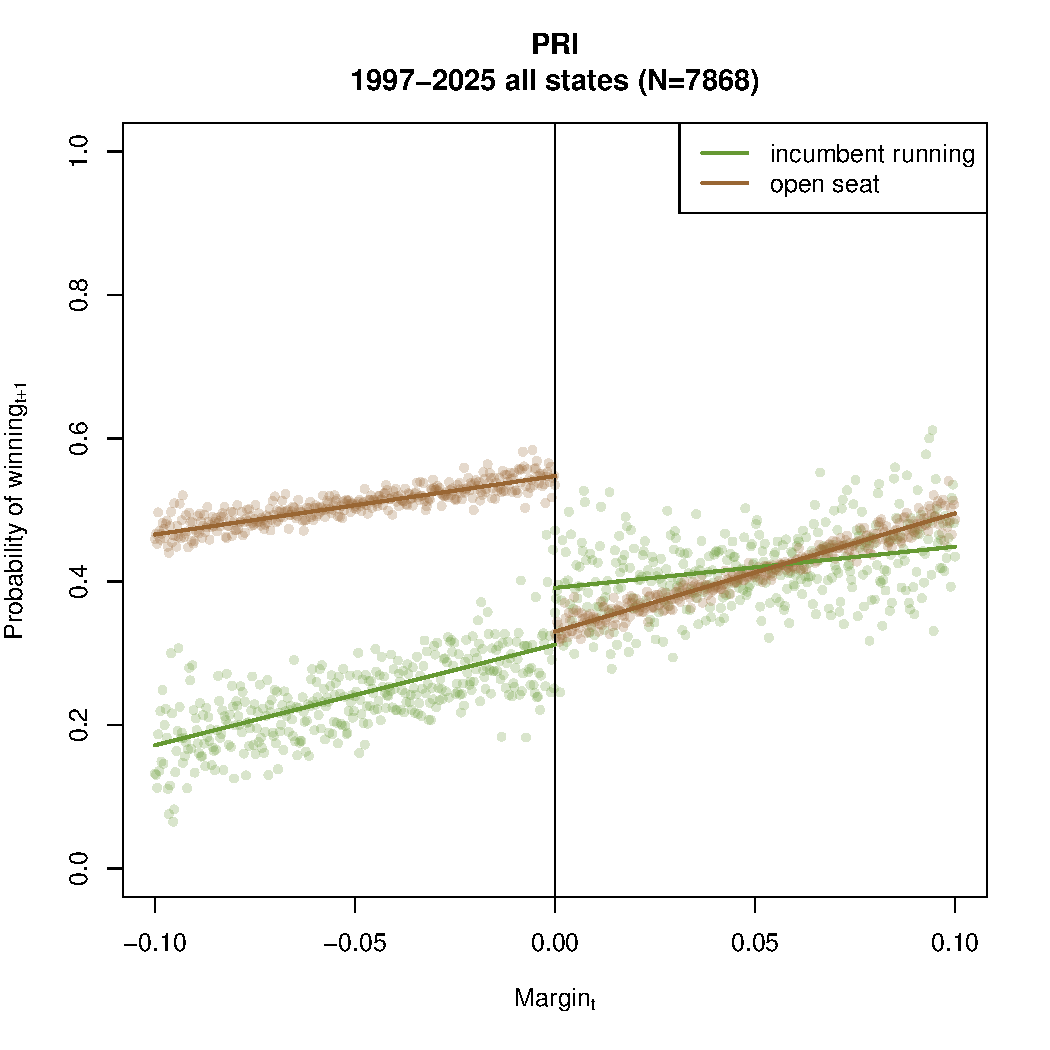
\includegraphics[width=.31\columnwidth]{../plots/pri4ALLmcmc.pdf} \\
  %% \end{tabular}
  \begin{tabular}{cc}
  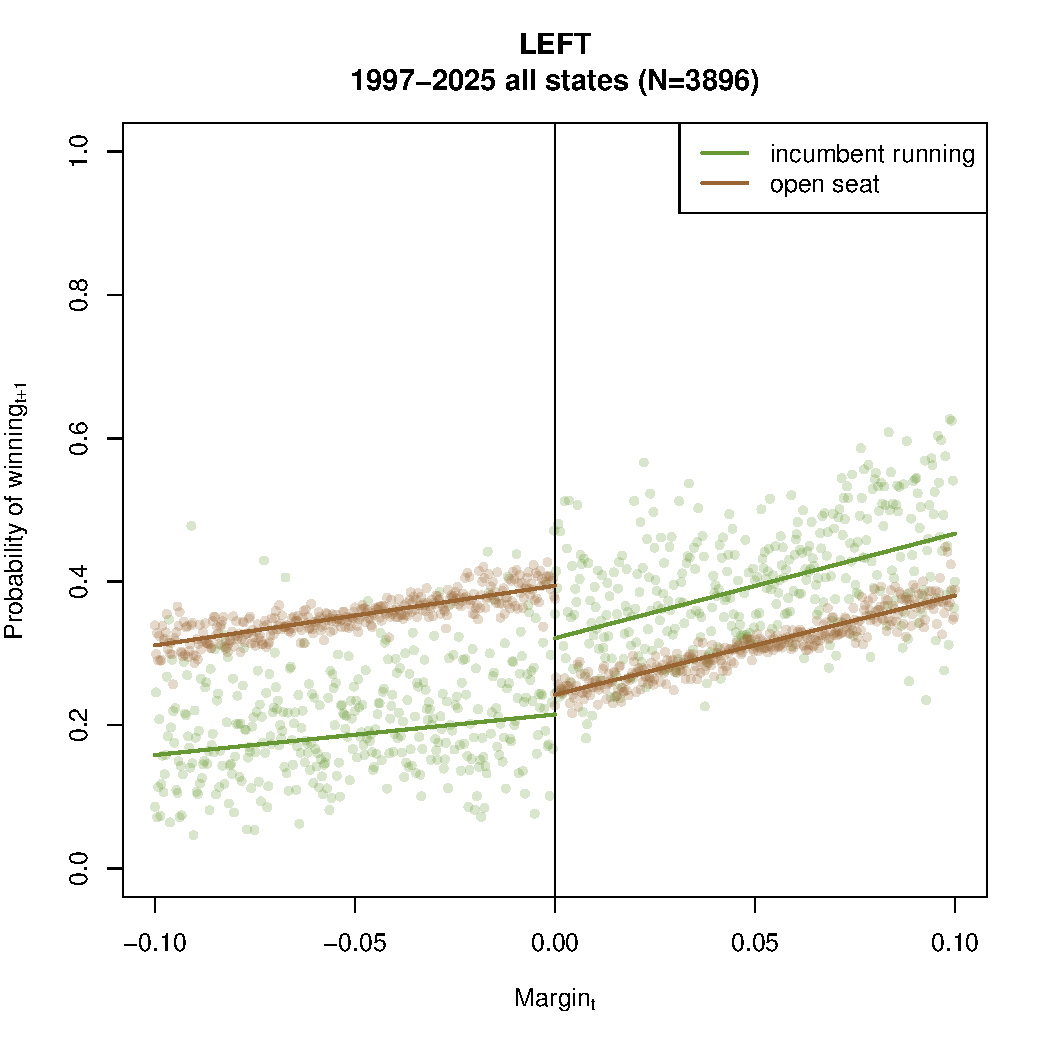
\includegraphics[width=.48\columnwidth]{../plots/left4ALLmcmc.pdf} &
  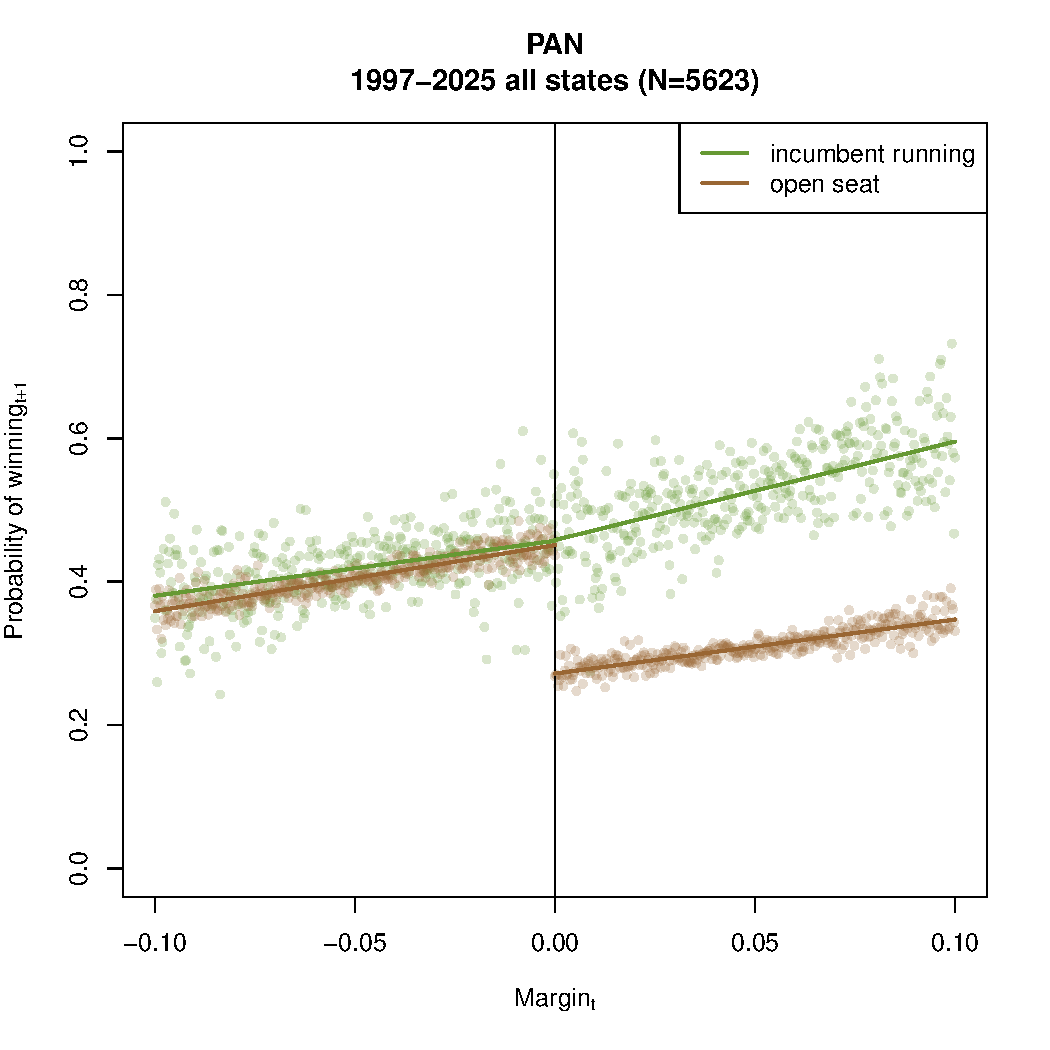
\includegraphics[width=.48\columnwidth]{../plots/pan4ALLmcmc.pdf} \\
  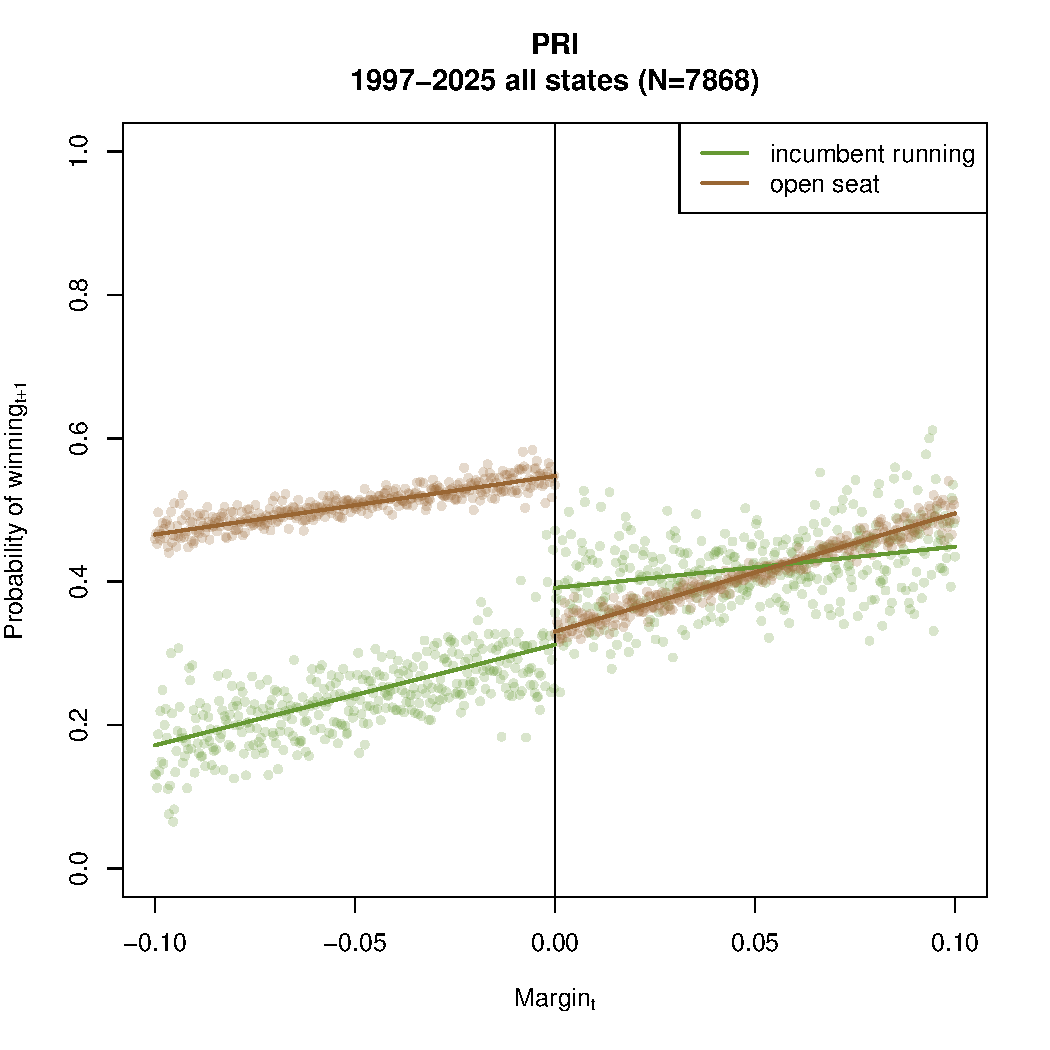
\includegraphics[width=.48\columnwidth]{../plots/pri4ALLmcmc.pdf} \\
  \end{tabular}
  \caption{Simulaciones con datos del periodo 1997--2025. Método MCMC de estimación de la equación 1.}\label{F:full}
  %\caption{Simulations with the full 1997--2025 data. MCMC method of estimation of Equation (1).}
\end{figure}

% Destaca la amplitud de su brecha de ordenadas al origen marrón, de alrededor de 40 en vez de 20 puntos, así como las pendientes más pronunciadas. La erosión del partido presidencial en elecciones intermedias, en especial después de una elección crítica como fue 2018, dejó especialmente vulnerables los triunfos de Morena en municipios que AMLO arrastró a una victoria muy marginal. Un margen de +1 punto porcentual en vez de +5 redujo la probabilidad de reelección del Morena de 0.4 a 0.2; un margen de --1, en cambio, la elevó hasta 0.6.

The green portion of the diagram, by contrast, corresponds to municipal elections in which the incumbent mayor sought consecutive reelection. Three patterns stand out.

\begin{enumerate}

\item It is notable how the gap in the intercepts reverses. In statistical terms, it rather dissolves: if we estimated a single green regression line for both negative and positive margins, it would yield results almost identical to those reported.%\footnote{In 100 percent of the posterior samples there is a cursed gap for the mayor’s party when the incumbent is not on the ballot ($\beta_0 < \alpha_0$). By contrast, there is a reversed gap when the incumbent is on the ballot ($\beta_0 + \beta_1 > \alpha_0 + \alpha_1$) in between 15 and 20 percent of the posterior sample.}

\item In the right quadrant of each diagram one can distinguish, despite the noise in the cloud of green points, that static ambition doubles the probability that the PAN and the left win in $t+1$. For the PRI, which after the reform also lost its status as the dominant municipal party, the clouds overlap.

\item The left quadrants are the counterpart to the relative stability introduced by consecutive reelection. It becomes more difficult for all three parties to defeat an opposition mayor who appears on the ballot.

\end{enumerate}

\begin{figure}
  \centering
  \begin{tabular}{cc}
    \textbf{Pre-banderazo} & \textbf{Post-banderazo} \\
  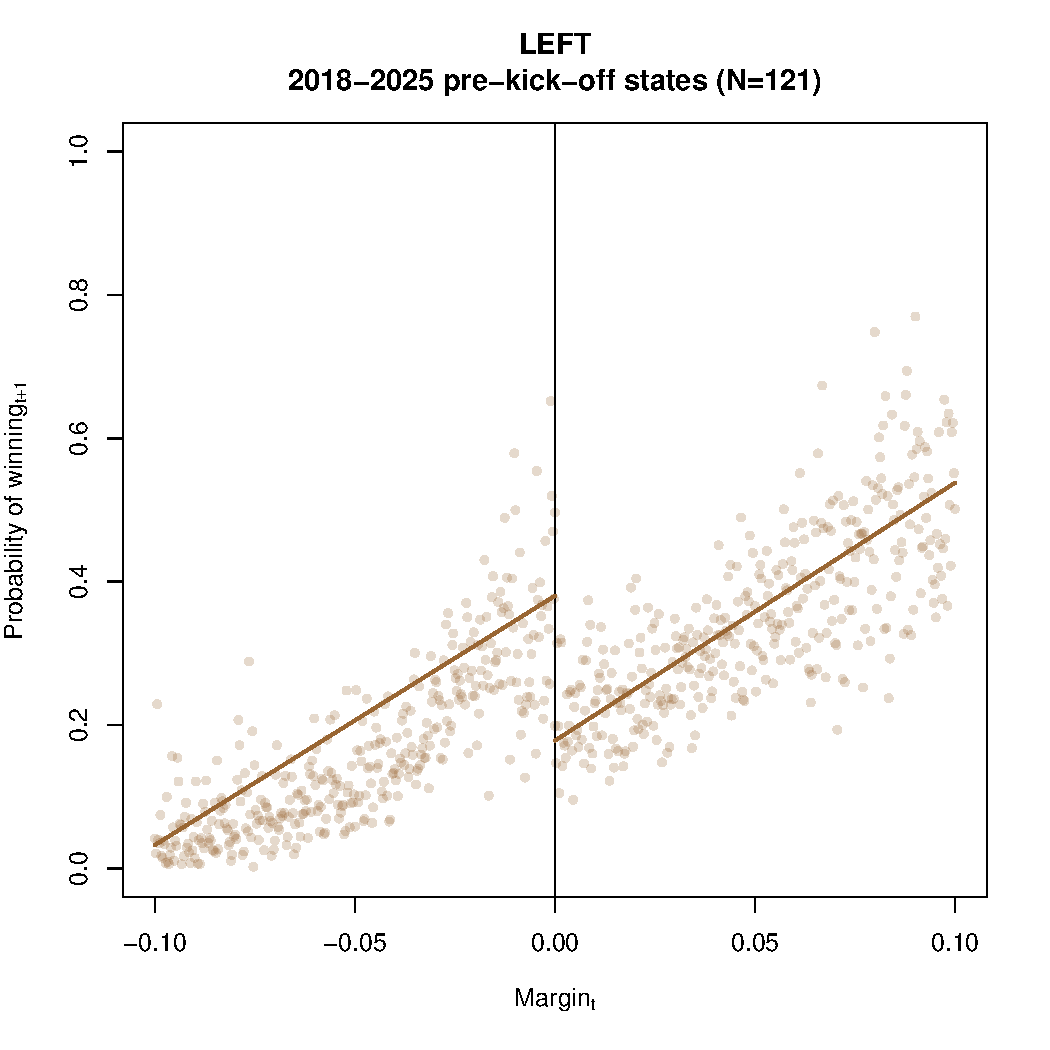
\includegraphics[width=.4\columnwidth]{../plots/left2PREKICKmcmc.pdf} &
  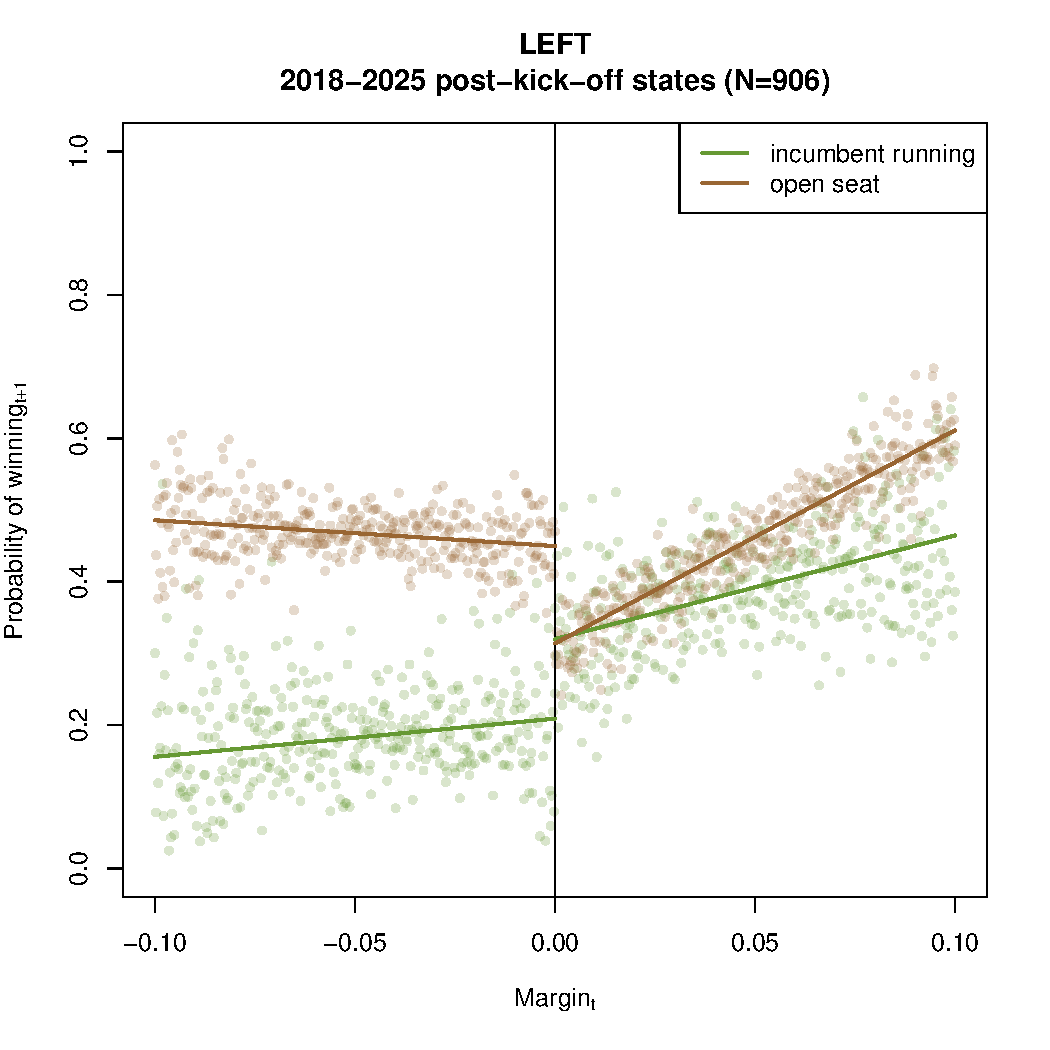
\includegraphics[width=.4\columnwidth]{../plots/left3POSTKICKmcmc.pdf} \\
  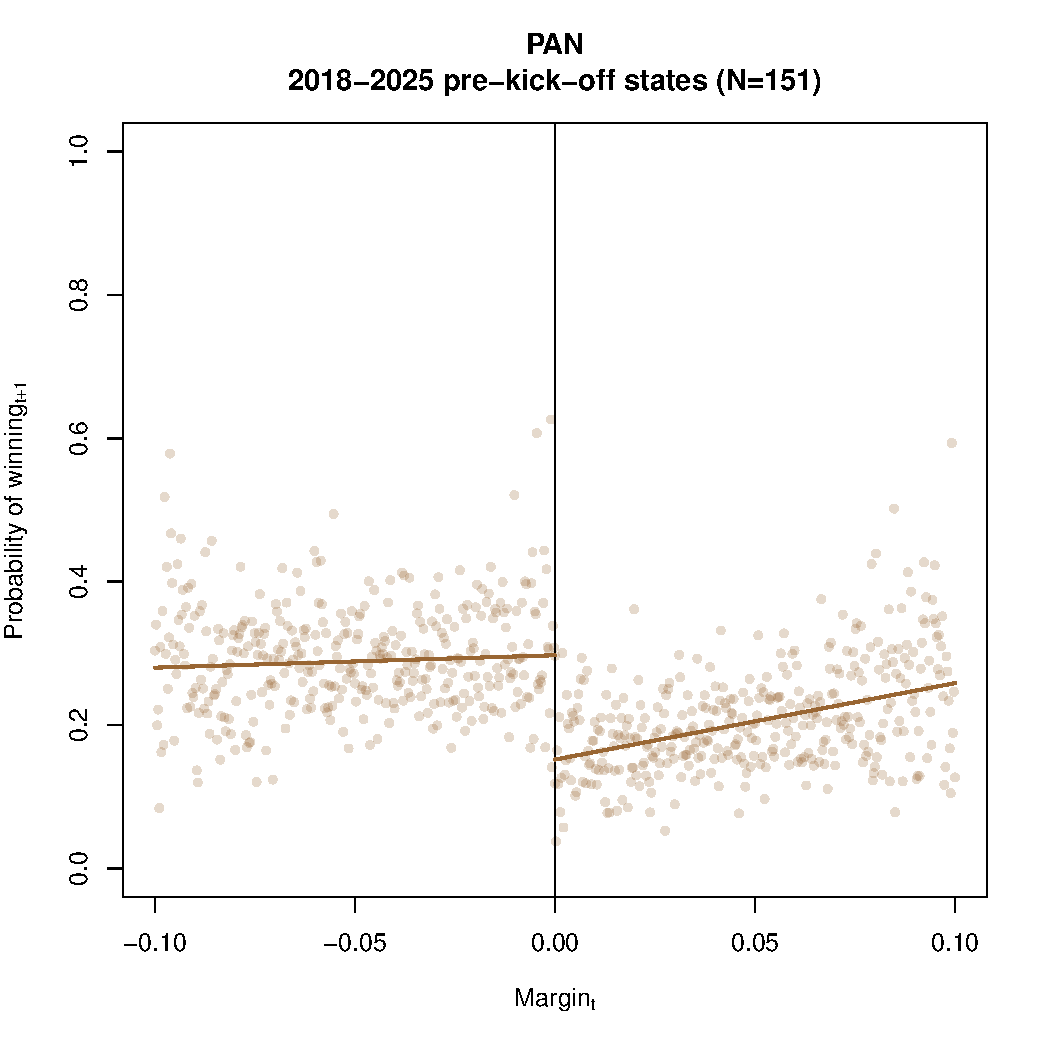
\includegraphics[width=.4\columnwidth]{../plots/pan2PREKICKmcmc.pdf} &
  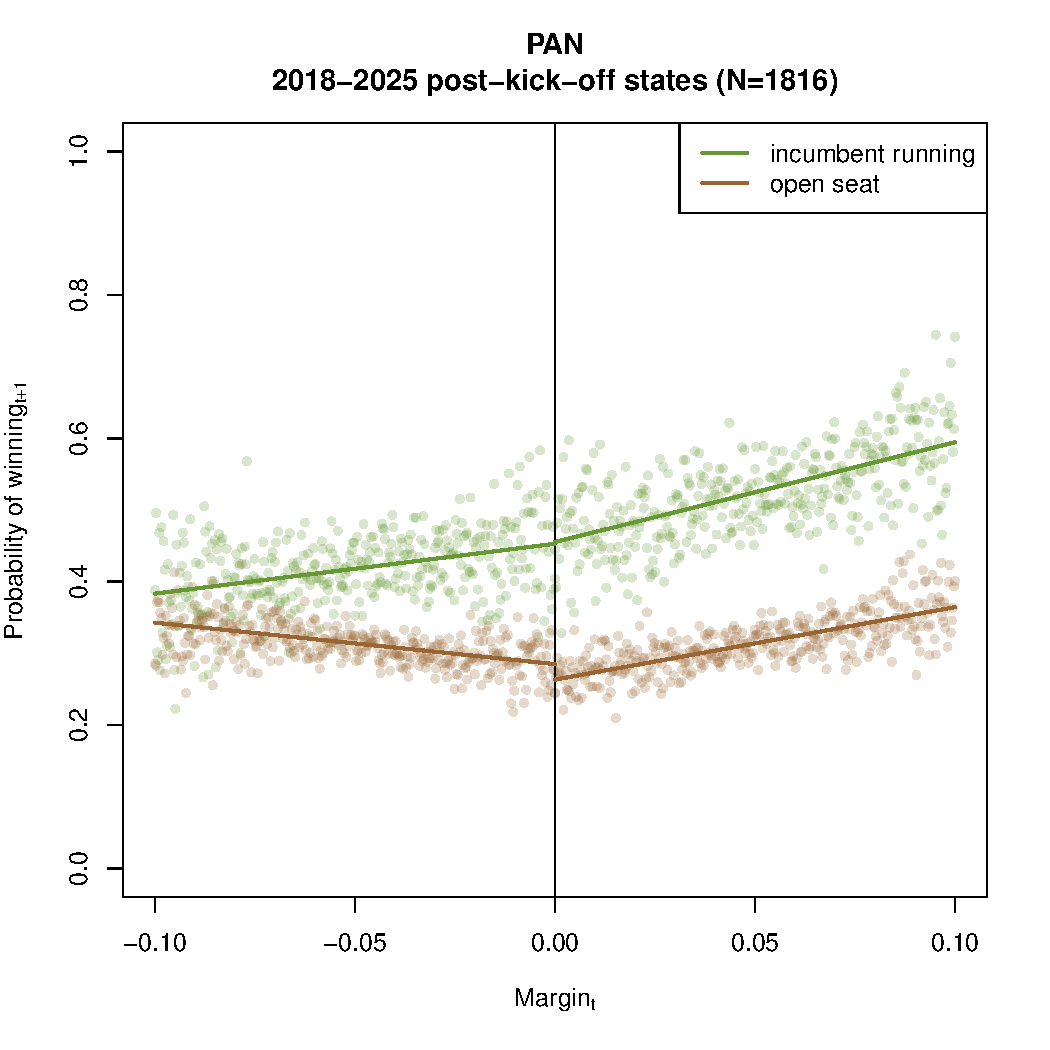
\includegraphics[width=.4\columnwidth]{../plots/pan3POSTKICKmcmc.pdf} \\
  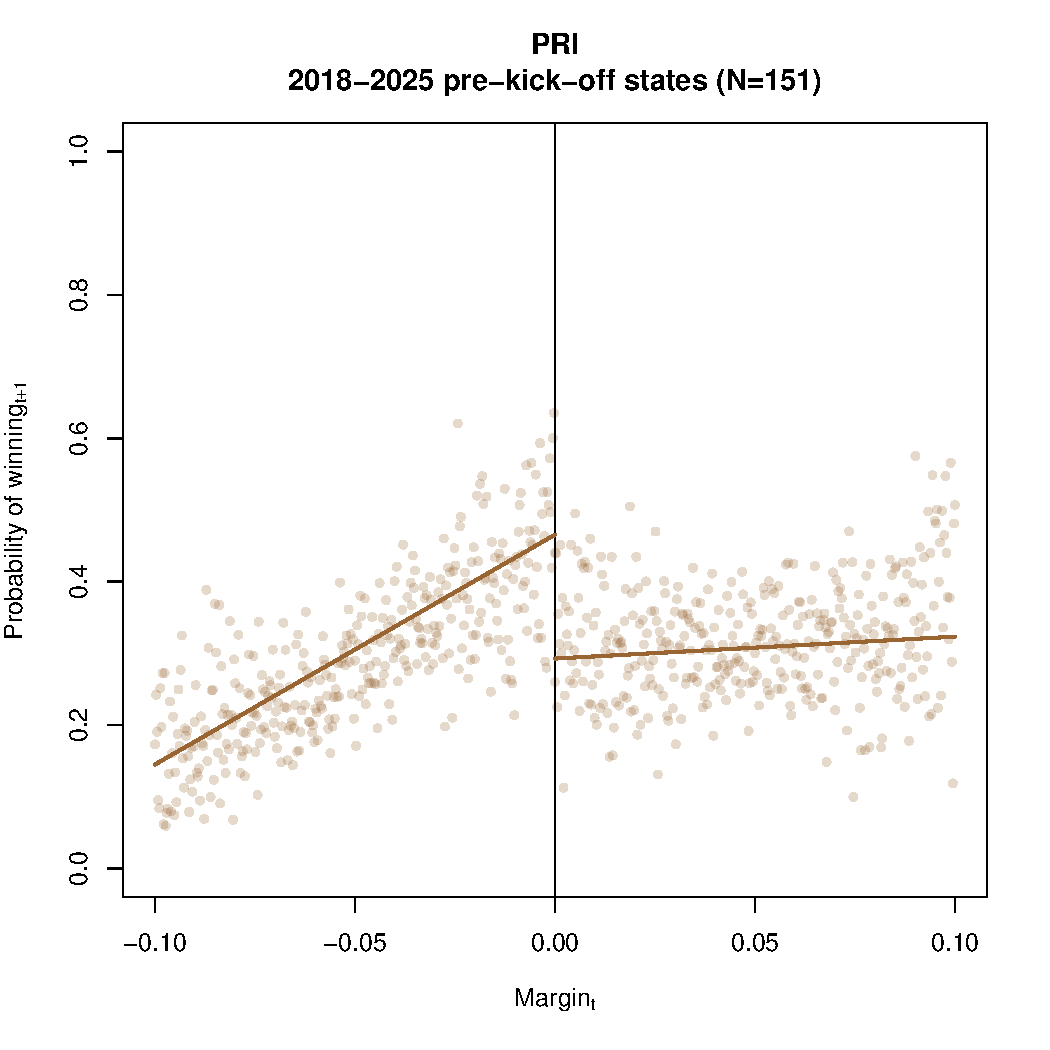
\includegraphics[width=.4\columnwidth]{../plots/pri2PREKICKmcmc.pdf}  &
  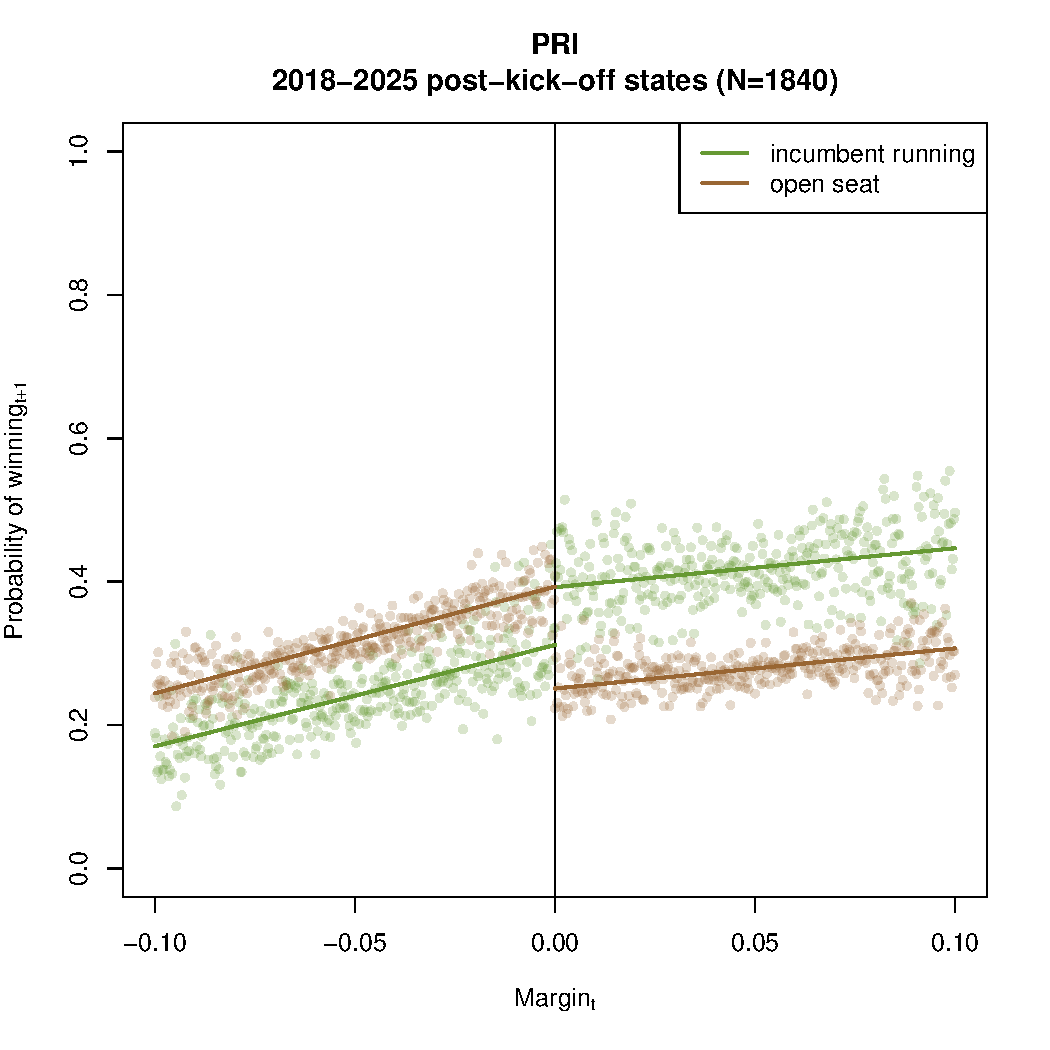
\includegraphics[width=.4\columnwidth]{../plots/pri3POSTKICKmcmc.pdf} \\
  \end{tabular}
  \caption{Simulations with the full 1997--2025 data. MCMC method of estimation of Equation (1).}
  %\caption{Simulaciones con datos del periodo 2018--2025. Método MCMC de estimación de la equación 1.}\label{F:2018-25}
\end{figure}

The key point: the curse of the incumbent party disappears when the mayor runs for reelection. Table \ref{T:posteriors} reports samples from the posterior distribution of several parameters of interest in the model. In every case the direction of the anti-incumbent gap reverses, although with mixed evidence. With an open seat, $\beta_0 < \alpha_0$ in the entirety of the 1,500 posterior samples from the estimations. By contrast, when the municipal president seeks reelection, $\beta_0 + \beta_1 < \alpha_0 + \alpha_1$ in only one-fifth or less of the posterior sample. The gap reverses four out of five times. This is no small matter. A mayor on the ballot acts as an insurance policy against negative partisan \emph{swings}.

\begin{table}
  \centering
  \begin{tabular}{clccr}
   &                   &   Curse gap when no        &         Curse gap when                     &       \\
   &                   & incumbent was in the ticket &        incumbent was in the ticket          &       \\ 
   & Party   & ($\alpha_0 > \beta_0$) & ($\alpha_0 + \alpha_1) > (\beta_0 + \beta_1$) & $N$      \\[-1.5ex] \\ \hline \\[-1.5ex] 
   %% &                   &      brecha sin       &                 brecha con                  &       \\
   %% &                   & ocupante en la boleta &            ocupante en la boleta            &       \\ 
   %% & Partido & ($\alpha_0 > \beta_0$) & ($\alpha_0 + \alpha_1) > (\beta_0 + \beta_1$) & $N$      \\[-1.5ex] \\ \hline \\[-1.5ex] 
   & \mc{3}{l}{~\textbf{1997--2017 all municipalities}} \\
   %% & \mc{3}{l}{~\textbf{1997--2017 todos los municipios}} \\
$a$& Left              &         1.000         &                    ---                      & 2,869 \\
$b$& PAN               &         1.000         &                    ---                      & 3,656 \\
$c$& PRI               &         1.000         &                    ---                      & 5,877 \\ \\[-1.5ex]
   & \mc{3}{l}{~\textbf{2018--2025 pre-kick-off municipalities}} \\
   %% & \mc{3}{l}{~\textbf{2018--2025 municipios pre-banderazo}} \\
$d$& Morena            &         0.916         &                    ---                      &   121 \\
$e$& PAN               &         0.876         &                    ---                      &   151 \\
$f$& PRI               &         0.858         &                    ---                      &   151 \\ \\[-1.5ex]
   & \mc{3}{l}{~\textbf{2018--2025 non-reform municipalities (Hidalgo \& Veracruz)}} \\
   %% & \mc{3}{l}{~\textbf{2018--2025 municipios de Hidalgo y Veracruz}} \\
$g$& Morena            &         0.889         &                    ---                      &   111 \\
$h$& PAN               &         0.075         &                    ---                      &   199 \\
$i$& PRI               &         0.605         &                    ---                      &   169 \\ \\[-1.5ex]
   & \mc{3}{l}{~\textbf{2018--2025 post-kick-off municipalities}} \\
   %% & \mc{3}{l}{~\textbf{2018--2025 municipios post-banderazo}} \\
$j$& Morena            &         0.984         &                    0.219                    &   906 \\
$k$& PAN               &         0.677         &                    0.488                    & 1,816 \\
$l$& PRI               &         0.999         &                    0.177                    & 1,840 \\ \\[-1.5ex]
   & \mc{3}{l}{~\textbf{1997--2025 all municipalities}} \\
   %% & \mc{3}{l}{~\textbf{1997--2025 todos los municipios}} \\
$m$& Left              &         1.000         &                    0.225                    & 3,896 \\
$n$& PAN               &         1.000         &                    0.504                    & 5,623 \\
$o$& PRI               &         1.000         &                    0.189                    & 7,868 \\[-1.5ex] \\ \hline
  \end{tabular}
  \caption{Hypothesis tests. Cells report the proportion of the posterior sample meeting the hypothesized inequality.}\label{T:posteriors}
  %% \caption{Pruebas de hipótesis. Las celdas reportan la proporción de la muestra posterior que cumple la hipótesis.}\label{T:posteriors}
\end{table}

The estimation of models with data subsets for the 2018--2025 period appears in Table \ref{T:regs} and Figure \ref{F:regplot}. These are still very preliminary models, but they distinguish close municipal elections in states that had not yet given the initial kick-off (models 1, 2, and 3) from those in states that had already done so (models 4, 5, and 6). These are linear probability models of equation 1.\footnote{That is, they are linear regressions with a dichotomous dependent variable. In my experience, the estimates of these models always coincide with the more refined estimates of logit models, and they allow a direct reading of the marginal effects. The intention is to replace them with logit models and to perform Bayesian estimations like those reported above.}

\begin{table}
  \centering
  \begin{tabular}{@{\extracolsep{5pt}}lcccccc}
    \\[-1.8ex]\hline 
    \hline \\[-1.8ex] 
    %% & \mc{3}{c}{Pre-banderazo inicial} & \mc{3}{c}{Post-banderazo inicial} \\ \cline{2-4} \cline{5-7}
    & \mc{3}{c}{Pre-kick-off} & \mc{3}{c}{Post-kick-off} \\ \cline{2-4} \cline{5-7}
    & (1) & (2) & (3) & (4) & (5) & (6) \\ 
    Variable  & Morena & PAN & PRI & Morena & PAN & PRI \\
    \hline \\[-1.8ex] 
    \mc{2}{l}{\textbf{When $\text{neg}_t=1$}} & & & & & \\
    Intercept & 0.338$^{***}$ & 0.303$^{***}$ & 0.451$^{***}$ &  0.450$^{***}$ & 0.284$^{***}$ & 0.390$^{***}$ \\
    &       (0.100) &       (0.092) &       (0.097) &        (0.047) &       (0.034) &       (0.034) \\
    & & & & & & \\ [-2.5ex]
    inc$_{t+1}$  &               &               &               & $-$0.230$^{*}$ &  0.169$^{**}$ &      $-$0.081 \\
    &               &               &               &        (0.127) &       (0.070) &       (0.065) \\
    & & & & & & \\ [-2.5ex]
    mg$_{t}$  &   3.438$^{*}$ &         0.128 &   3.186$^{*}$ &       $-$0.339 &      $-$0.589 &  1.483$^{**}$ \\
    &       (1.921) &       (1.742) &       (1.893) &        (0.905) &       (0.627) &       (0.625) \\
    & & & & & & \\ [-2.5ex]
    mg$_{t}\times$inc$_{t+1}$ &               &               &               &          0.859 &         1.301 &      $-$0.076 \\
    &               &               &               &        (2.305) &       (1.304) &       (1.205) \\
    \mc{2}{l}{\textbf{When $\text{neg}_t=0$}} & & & & & \\
    Intercept &   0.174$^{*}$ &   0.154$^{*}$ & 0.292$^{***}$ &  0.311$^{***}$ & 0.263$^{***}$ & 0.250$^{***}$ \\
    &       (0.094) &       (0.084) &       (0.102) &        (0.050) &       (0.034) &       (0.033) \\
    & & & & & & \\ [-2.5ex]
    inc$_{t+1}$    &               &               &               &          0.012 & 0.193$^{***}$ &  0.143$^{**}$ \\
    &               &               &               &        (0.112) &       (0.073) &       (0.071) \\
    & & & & & & \\ [-2.5ex]
    mg$_{t}$     &   3.480$^{*}$ &         1.059 &         0.409 &  2.952$^{***}$ &         0.987 &         0.559 \\
    &       (1.874) &       (1.756) &       (1.999) &        (0.932) &       (0.628) &       (0.602) \\
    & & & & & & \\ [-2.5ex]
    mg$_{t}\times$inc$_{t+1}$  &               &               &               &       $-$1.537 &         0.374 &      $-$0.036 \\
    &               &               &               &        (2.049) &       (1.338) &       (1.296) \\
    & & & & & & \\ [-2.5ex]
    \hline \\[-1.8ex] 
    R$^2$          &         0.311 &         0.258 &         0.325 &          0.451 &         0.361 &         0.315 \\
    Observations   &           121 &           151 &           151 &            906 &         1,816 &         1,840 \\
    & & & & & & \\ [-2.5ex]
    %% \hline \\[-1.8ex]
    %% \mc{3}{l}{Wald tests (p-values)} \\
    %% $\alpha_0 = \beta_0$ & 0.067 & 0.069 & 0.004 & $<$0.001 & $<$0.001 & $<$0.001 \\
    %% $\alpha_0 + \alpha_2 = \beta_0 + \beta_2$ & & & & $<$0.001 & $<$0.001 & $<$0.001 \\
    %% \\[-1.8ex]
    \hline 
    \hline \\[-1.8ex] 
  \end{tabular}
  \caption{Six marginal election models in the 2018--2025 period. `Pre-kick-off' models include only municipalities in states where the reelection reform was not yet adopted, `post-kick-off' only municipalities in the remainder states. The dependent variable in all models is the party's reelection indicator in $t+1$, fitting linear probability models with OLS. \textit{Note:} $^{*}$p$<$0.1; $^{**}$p$<$0.05; $^{***}$p$<$0.01.}\label{T:regs}
%%  \caption{Seis modelos de elecciones marginales para el periodo 2018--2025. Los modelos `pre-banderazo' incluyen sólo municipios en estados donde aún no entraba en vigor la reforma reeleccionista, los `post-banderazo' sólo municipios donde ya estaba en vigor. La variable dependiente en todos los casos es el indicador de reelección del partido en $t+1$, estimando modelos de probabilidad lineal con OLS. \textit{Nota:} $^{*}$p$<$0.1; $^{**}$p$<$0.05; $^{***}$p$<$0.01.}\label{T:regs}
\end{table}

%% #+CAPTION: Fortunas del partido municipal en elecciones marginales con/sin ocupante en la boleta
%% #+NAME:   fig:2
%% | file:../assets/img/left-97-23-mcmc.png | file:../assets/img/left-18-23-mcmc.png |
%% | file:../assets/img/pan-97-23-mcmc.png  | file:../assets/img/pan-18-23-mcmc.png  |
%% | file:../assets/img/pri-97-23-mcmc.png  | file:../assets/img/pri-18-23-mcmc.png  |

I will not dwell now on discussing the estimates reported in the table, in order to focus on the simulations in Figure \ref{F:regplot}. The results do not yet report uncertainty, only point estimates, but they corroborate the patterns observed above. In the period since 2018, in close elections prior to the reform kickoff, anti-incumbent party gaps are evident on the left side of the diagram. The right column, showing close elections after the kickoff, displays more differentiated patterns, but one can observe a fading (for the PAN) or even a reversal (for the PRI and especially Morena) of the incumbent party curse when the mayor appears on the ballot.

\begin{figure}
  \centering
  \resizebox{.8\textwidth}{!}{
    \begin{tabular}{cc}
      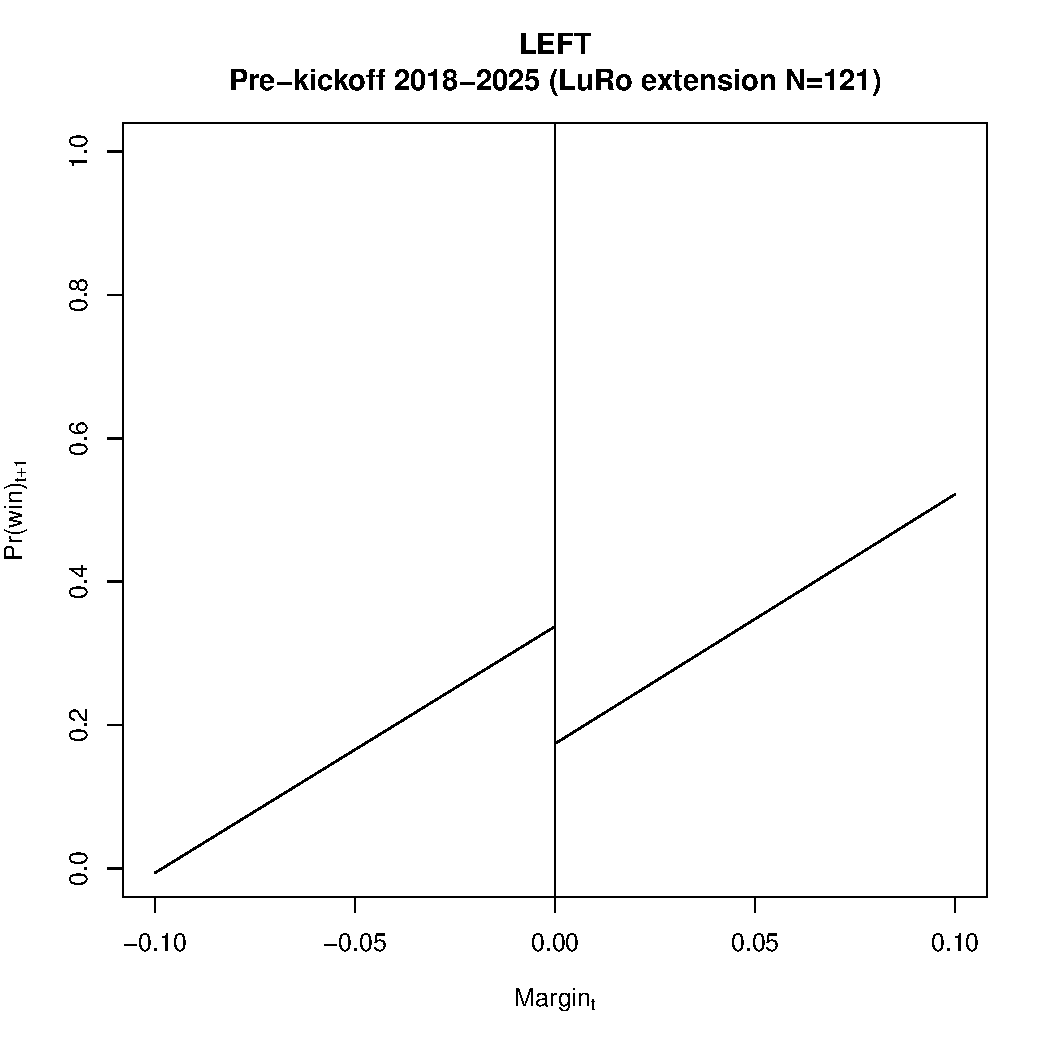
\includegraphics[width=.45\columnwidth]{../plots/leftPREKICKlpm.pdf} &
      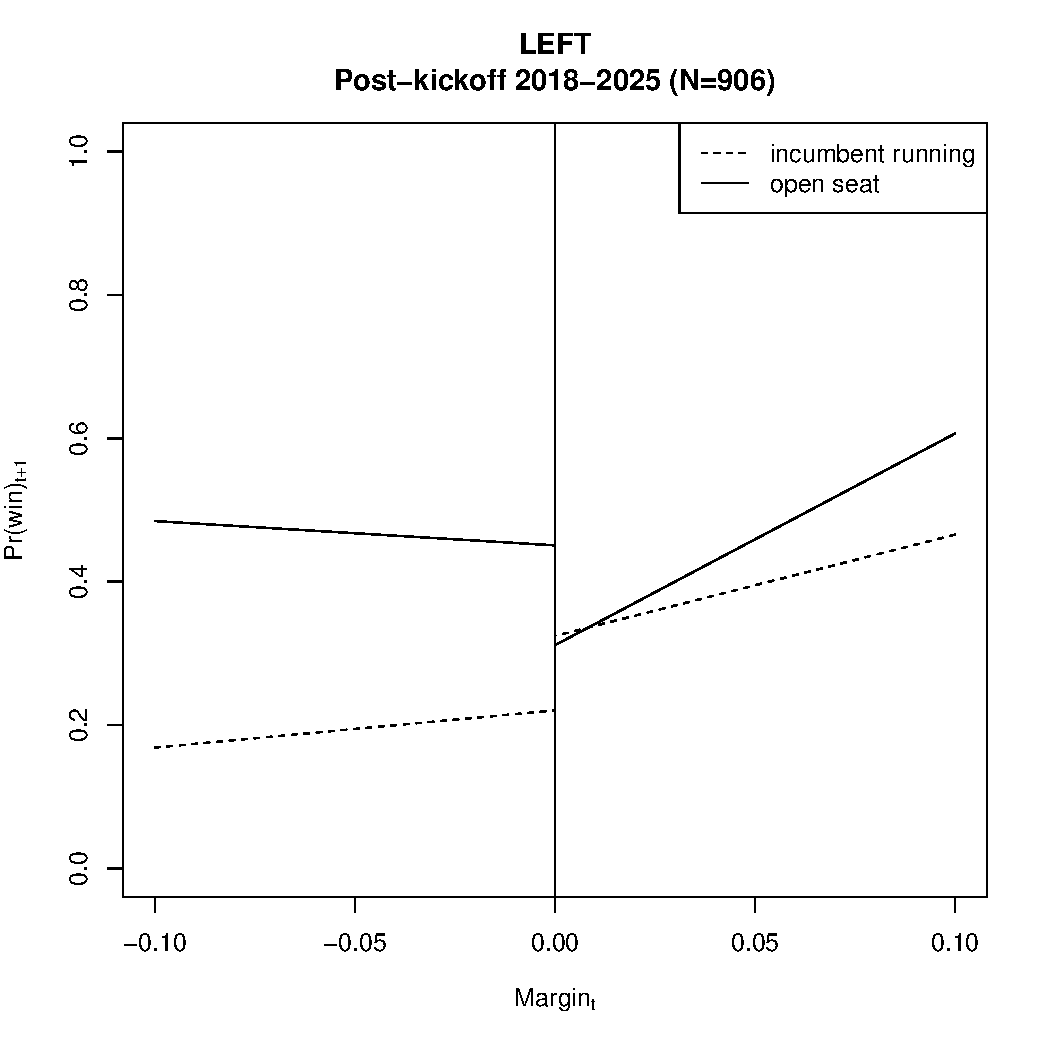
\includegraphics[width=.45\columnwidth]{../plots/leftPOSTKICKlpm.pdf} \\
      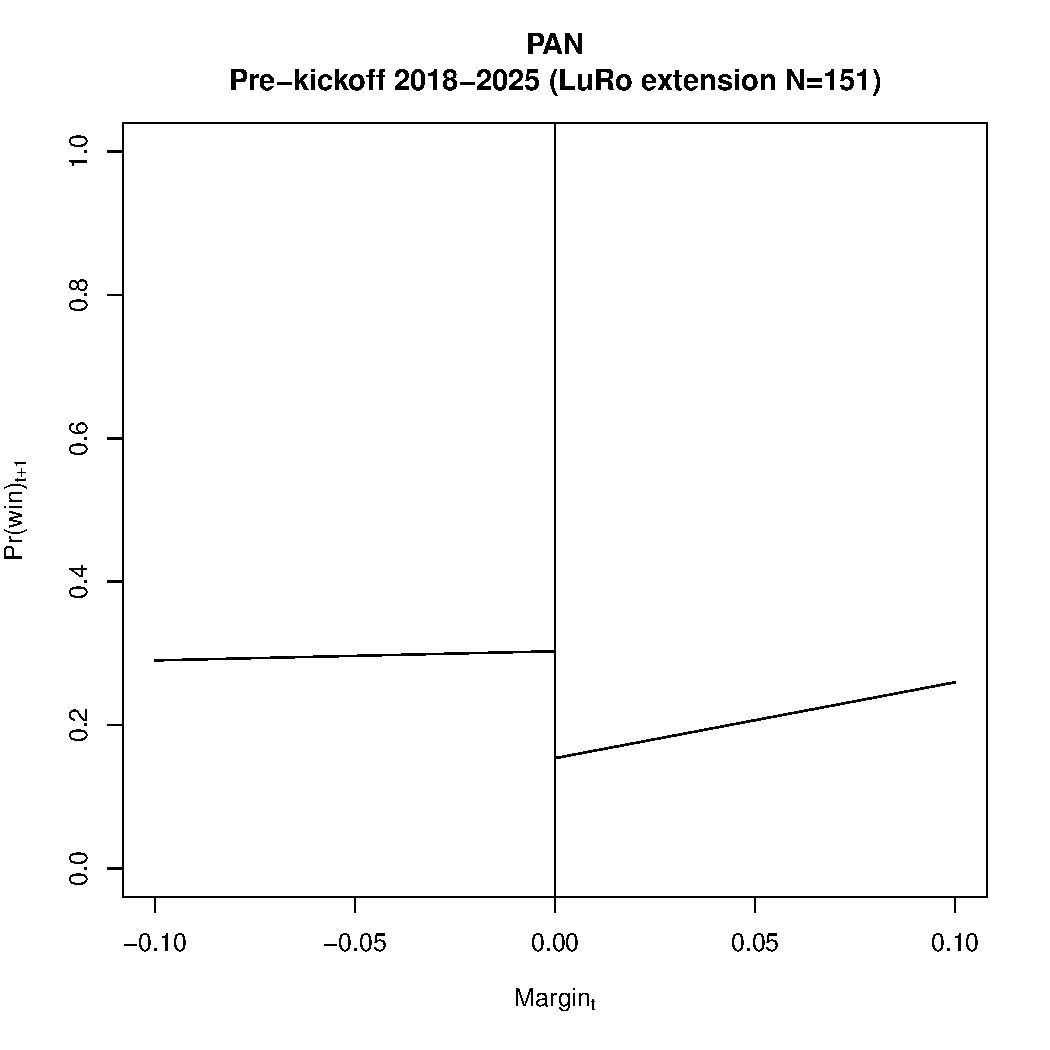
\includegraphics[width=.45\columnwidth]{../plots/panPREKICKlpm.pdf} &
      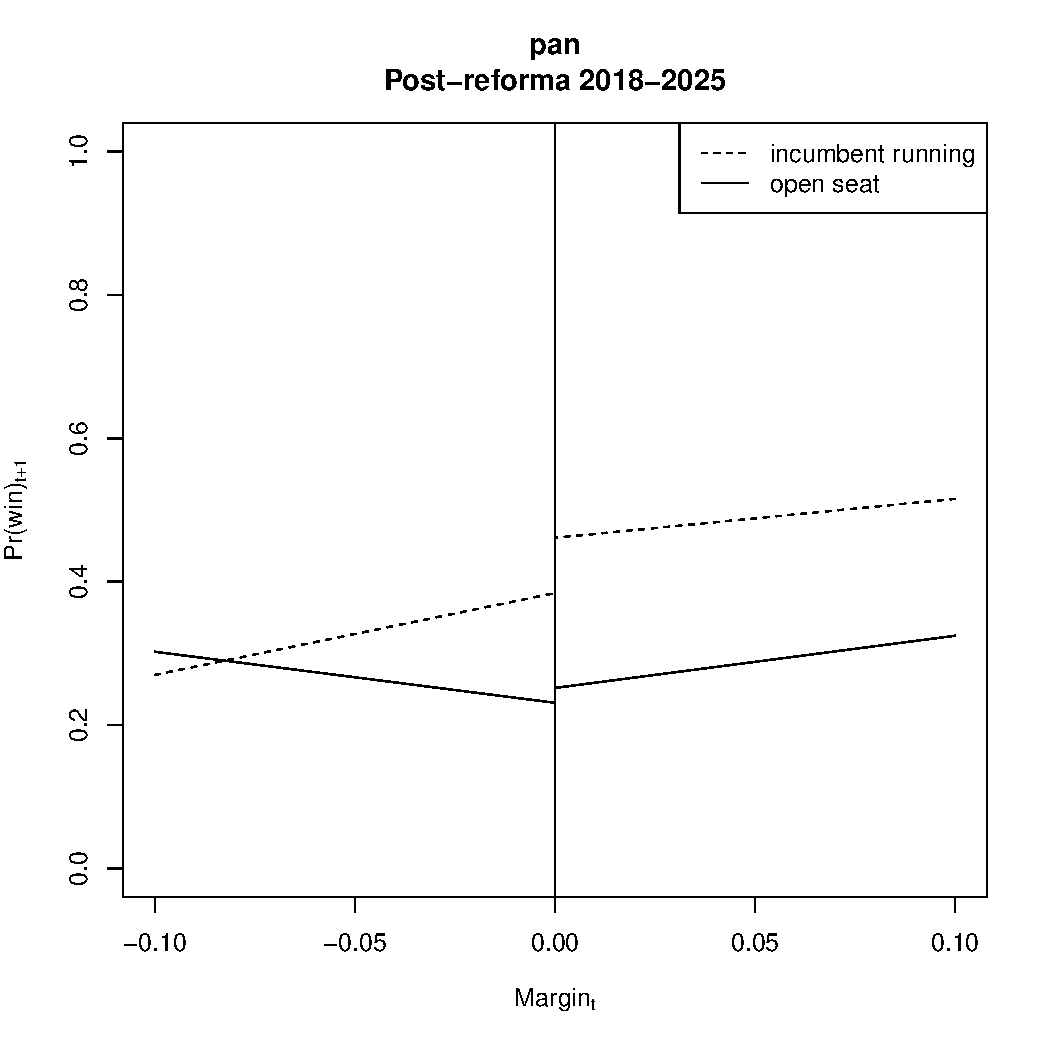
\includegraphics[width=.45\columnwidth]{../plots/panPOSTKICKlpm.pdf} \\
      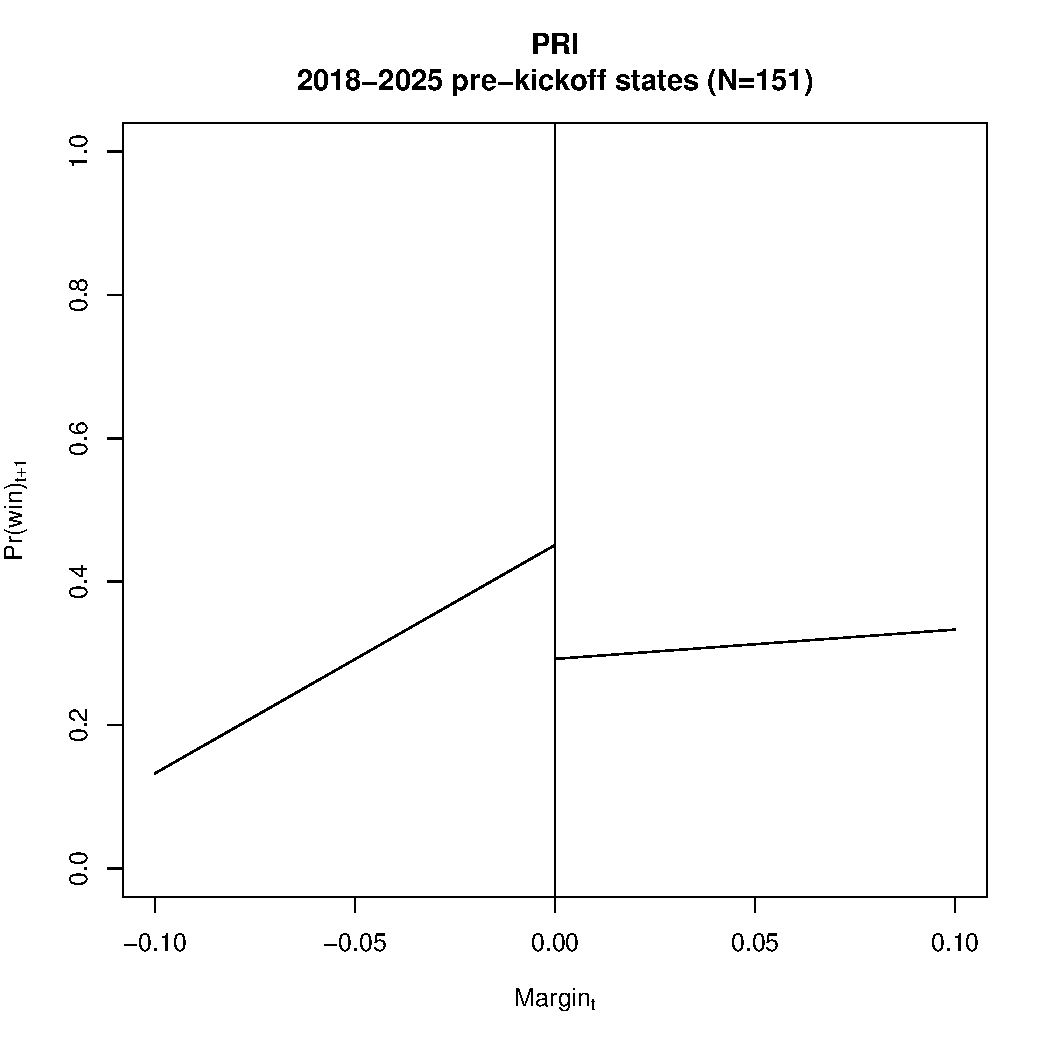
\includegraphics[width=.45\columnwidth]{../plots/priPREKICKlpm.pdf} &
      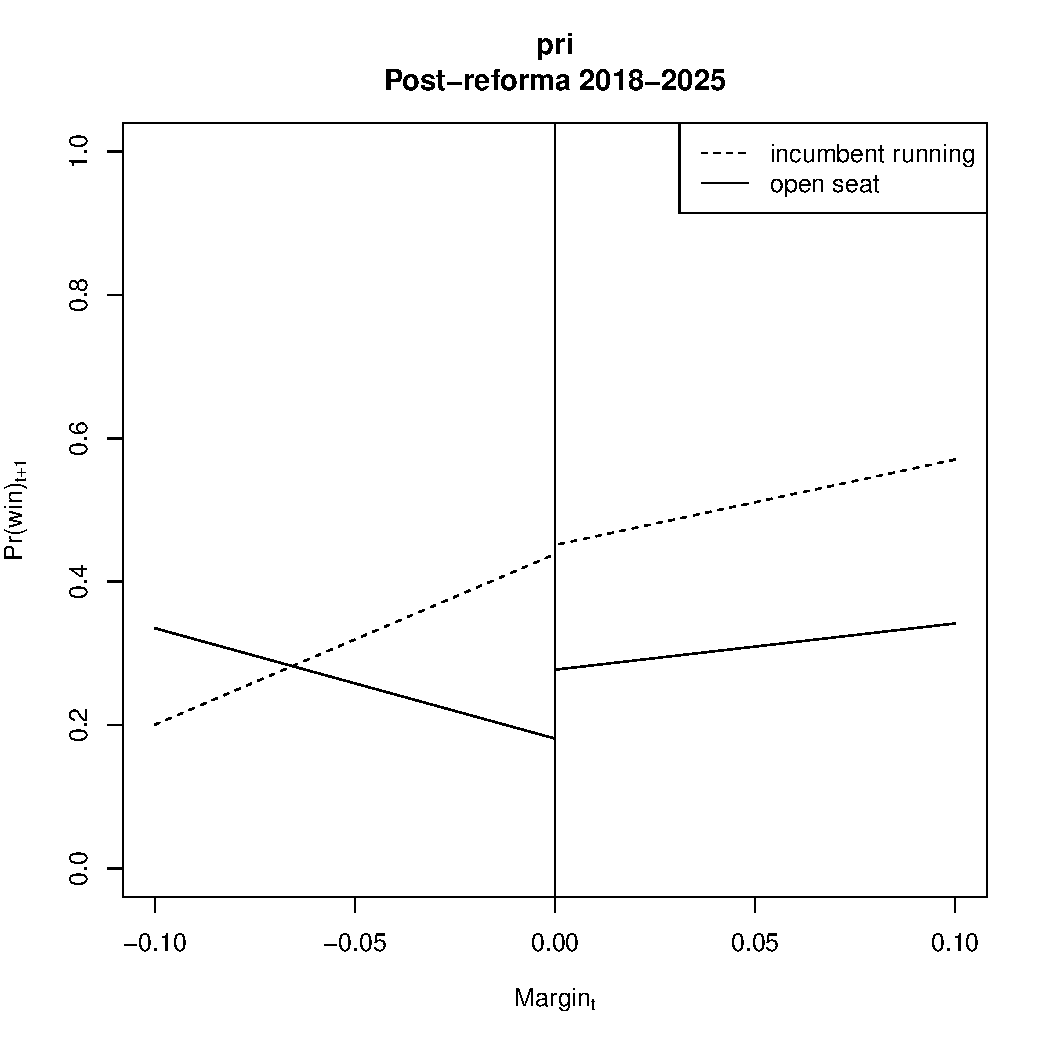
\includegraphics[width=.45\columnwidth]{../plots/priPOSTKICKlpm.pdf} \\
    \end{tabular}
  }
  %^\caption{The effect of the election margin on the future probability of reelection}\label{F:regplot}
  \caption{El efecto del margen electoral en la probabilidad de reelección partidista futura. Simulaciones con los modelos 1, 2 y 3 en la columna izquierda, con los modelos 4, 5 y 6 en la columna derecha.}\label{F:regplot}
\end{figure}  

\section{Conclusion}

\noindent TBW

\newpage

\section{Appendix}

\subsection{Model for MCMC estimation}

\begin{scriptsize}
\begin{verbatim}
library(R2jags)
logitModel <- function() {
    ### linear probability model with logit link
    for (n in 1:N){                ## loop over observations
        depvar[n] ~ dbern(p[n]);   
        logit(p[n]) <- inprod(beta[],X[n,]);
    }
    ############################
    ## NON-INFORMATIVE PRIORS ##
    ############################
    for (k in 1:K){                ## loop over regressors
        beta[k] ~ dnorm(0, .0001);
    }
}
depvar <- data$dwin
N <- length(depvar)
X <- data.frame(
    dneg=data$dneg       , dnegxincball=data$dnegxincball
  , dnegxmg=data$dnegxmg , dnegxmgxincball=data$dnegxmgxincball
  , dpos=data$dpos       , dposxincball=data$dposxincball
  , dposxmg=data$dposxmg , dposxmgxincball=data$dposxmgxincball
    )
##
K <- ncol(X)
X <- as.matrix(X)
### Data, initial values, and parameter vector for jags
dl.data <- list("N", "K", "depvar", "X")
dl.inits <- function (){
    list (
    beta=rnorm(K)
    )
}
dl.parameters <- c("beta")
##
## estimate
fitjags <- jags (data=dl.data, inits=dl.inits, dl.parameters,
                  model.file=logitModel, n.chains=3,
                  n.iter=100000, n.thin=100
                  )
traceplot(fitjags) ## visually inspect posterior parameter convergence
\end{verbatim}
\end{scriptsize}

\subsection{Summary of MCMC estimates}

\begin{sidewaystable}
  \centering
  \resizebox{.7\textwidth}{!}{
\begin{tabular}{c|rcr|rcr|rcr}
          &  \mc{3}{c}{Left} & \mc{3}{c}{PAN} & \mc{3}{c}{PRI} \\
          &   point   & .95-interval & $\hat{R}$  &   point   & .95-interval & $\hat{R}$  &   point   & .95-interval & $\hat{R}$  \\ \hline
  \mc{5}{l}{~\textbf{Model 1: 1997--2017 all municipalities pre-reform}} \\ %% model1
$\alpha_0$&  $-0.503$ &    $(-0.70, -0.31)$ & 1.001 & $ 0.107$ &          $(-0.07, 0.28)$ & 1.001 & $ 0.338$ &           $(0.19, 0.47)$ & 1.002 \\
%%$\alpha_1$&  $ 0.159$ & $(-198.05, 201.16)$ & 1.001 & $-1.566$ &      $(-200.94, 183.33)$ & 1.002 & $ 3.109$ &      $(-193.92, 202.62)$ & 1.003 \\
$\alpha_2$&  $ 4.215$ &      $(0.45, 7.88)$ & 1.002 & $ 6.509$ &           $(3.24, 9.82)$ & 1.003 & $ 2.058$ &          $(-0.60, 4.82)$ & 1.003 \\
%%$\alpha_3$&  $-1.908$ & $(-196.29, 193.49)$ & 1.003 & $-0.233$ &      $(-191.44, 194.40)$ & 1.004 & $-0.519$ &      $(-199.78, 196.34)$ & 1.000 \\
 $\beta_0$&  $-1.241$ &    $(-1.47, -1.01)$ & 1.003 & $-0.939$ &         $(-1.13, -0.74)$ & 1.000 & $-0.605$ &         $(-0.74, -0.46)$ & 1.000 \\
%% $\beta_1$&  $ 0.042$ & $(-198.29, 195.77)$ & 1.001 & $-3.166$ &      $(-191.44, 191.29)$ & 1.001 & $-1.575$ &      $(-210.59, 188.00)$ & 1.000 \\
 $\beta_2$&  $ 4.314$ &     $(-0.01, 8.35)$ & 1.001 & $ 2.895$ &          $(-0.47, 6.50)$ & 1.001 & $ 7.566$ &          $(5.19, 10.05)$ & 1.000 \\
%% $\beta_3$&  $ 0.213$ & $(-188.78, 197.53)$ & 1.002 & $-1.035$ &      $(-205.07, 195.70)$ & 1.002 & $ 3.274$ &      $(-199.57, 186.14)$ & 1.002 \\
deviance  &  $3475.1$ &    $(3471.6, 3482.6)$ & 1.002 & $4763.3$ &         $(4759.8, 4770.3)$ & 1.007 & $8029.9$ &         $(8026.5, 8036.6)$ & 1.001 \\
  \mc{5}{l}{~\textbf{Model 2: 2018--2025 pre-kick-in municipalities}} \\ %% model2
$\alpha_0$&  $-0.463$ &     $(-1.61, 0.63)$ & 1.001 & $-0.860$ &          $(-1.75, 0.07)$ & 1.002 & $-0.138$ &          $(-1.02, 0.76)$ & 1.001 \\
%%$\alpha_1$&  $ 1.308$ & $(-192.12, 197.28)$ & 1.000 & $ 1.988$ &      $(-202.22, 206.28)$ & 1.000 & $-2.593$ &      $(-184.70, 196.64)$ & 1.003 \\
$\alpha_2$&  $29.878$ &     $(1.13, 62.15)$ & 1.000 & $ 0.845$ &        $(-15.85, 18.60)$ & 1.001 & $16.373$ &         $(-1.49, 36.84)$ & 1.003 \\
%%$\alpha_3$&  $-1.379$ & $(-209.16, 185.75)$ & 1.001 & $ 2.358$ &      $(-196.09, 207.43)$ & 1.000 & $-0.428$ &      $(-192.96, 188.68)$ & 1.000 \\
 $\beta_0$&  $-1.517$ &    $(-2.57, -0.53)$ & 1.001 & $-1.721$ &         $(-2.81, -0.77)$ & 1.001 & $-0.882$ &          $(-1.83, 0.06)$ & 1.001 \\
%% $\beta_1$&  $-1.584$ & $(-190.64, 196.94)$ & 1.001 & $-4.191$ &      $(-199.20, 192.73)$ & 1.001 & $ 2.317$ &      $(-188.12, 190.76)$ & 1.001 \\
 $\beta_2$&  $16.726$ &    $(-2.27, 36.46)$ & 1.001 & $ 6.668$ &        $(-13.00, 27.31)$ & 1.001 & $ 1.436$ &        $(-17.30, 19.56)$ & 1.002 \\
%% $\beta_3$&  $ 2.621$ & $(-190.53, 209.16)$ & 1.001 & $ 4.496$ &      $(-188.64, 200.48)$ & 1.000 & $-3.773$ &      $(-201.35, 183.81)$ & 1.000 \\
deviance  &  $ 132.1$ &      $(128.5, 139.0)$ & 1.002 & $ 169.7$ &           $(166.1, 176.3)$ & 1.001 & $ 188.4$ &           $(184.8, 195.7)$ & 1.003 \\
  \mc{5}{l}{~\textbf{Model 3: 2018--2025 post-kick-in municipalities}} \\ %% model3
$\alpha_0$&  $-0.202$ &     $(-0.56, 0.15)$ & 1.001 & $-0.920$ &         $(-1.24, -0.63)$ & 1.001 & $-0.435$ &         $(-0.73, -0.14)$ & 1.000 \\
$\alpha_1$&  $-1.130$ &     $(-2.45, 0.06)$ & 1.001 & $ 0.731$ &           $(0.12, 1.30)$ & 1.001 & $-0.358$ &          $(-0.98, 0.23)$ & 1.001 \\
$\alpha_2$&  $-1.448$ &     $(-8.70, 5.73)$ & 1.001 & $-2.693$ &          $(-8.36, 2.94)$ & 1.001 & $ 6.948$ &          $(0.89, 13.09)$ & 1.000 \\
$\alpha_3$&  $ 5.041$ &   $(-19.33, 29.06)$ & 1.000 & $ 5.557$ &         $(-5.70, 16.49)$ & 1.001 & $ 0.965$ &        $(-10.98, 13.05)$ & 1.001 \\
 $\beta_0$&  $-0.783$ &    $(-1.18, -0.38)$ & 1.004 & $-1.029$ &         $(-1.36, -0.71)$ & 1.001 & $-1.094$ &         $(-1.43, -0.78)$ & 1.005 \\
 $\beta_1$&  $ 0.028$ &     $(-0.95, 0.95)$ & 1.002 & $ 0.849$ &           $(0.19, 1.47)$ & 1.000 & $ 0.656$ &           $(0.01, 1.30)$ & 1.003 \\
 $\beta_2$&  $12.350$ &     $(5.03, 19.75)$ & 1.002 & $ 4.730$ &         $(-0.89, 10.67)$ & 1.003 & $ 2.794$ &          $(-2.60, 8.55)$ & 1.004 \\
 $\beta_3$&  $-6.231$ &   $(-23.32, 10.70)$ & 1.001 & $ 0.890$ &        $(-10.37, 12.08)$ & 1.001 & $-0.561$ &        $(-12.81, 11.22)$ & 1.005 \\
deviance  &  $1221.2$ &    $(1215.6, 1229.9)$ & 1.001 & $2307.0$ &         $(2300.8, 2316.7)$ & 1.000 & $2240.9$ &         $(2235.0, 2250.7)$ & 1.002 \\
  \mc{5}{l}{~\textbf{Model 4: 1997--2025 all municipalities}} \\ %% model4
$\alpha_0$&  $-0.429$ &    $(-0.60, -0.25)$ & 1.003 & $-0.197$ &         $(-0.34, -0.04)$ & 1.000 & $  0.190$ &           $(0.06, 0.31)$ & 1.002 \\
$\alpha_1$&  $-0.868$ &     $(-2.09, 0.27)$ & 1.000 & $ 0.025$ &          $(-0.54, 0.56)$ & 1.001 & $ -0.982$ &         $(-1.56, -0.45)$ & 1.003 \\
$\alpha_2$&  $ 3.657$ &      $(0.47, 6.90)$ & 1.003 & $ 3.841$ &           $(1.16, 6.55)$ & 1.000 & $  3.274$ &           $(0.92, 5.63)$ & 1.002 \\
$\alpha_3$&  $ 0.094$ &   $(-20.66, 22.80)$ & 1.004 & $-0.677$ &         $(-11.27, 9.83)$ & 1.001 & $  4.539$ &         $(-5.84, 15.80)$ & 1.003 \\
 $\beta_0$&  $-1.141$ &    $(-1.34, -0.95)$ & 1.001 & $-0.986$ &         $(-1.15, -0.82)$ & 1.000 & $ -0.707$ &         $(-0.83, -0.57)$ & 1.001 \\
 $\beta_1$&  $ 0.392$ &     $(-0.49, 1.21)$ & 1.002 & $ 0.817$ &           $(0.22, 1.37)$ & 1.003 & $  0.265$ &          $(-0.31, 0.84)$ & 1.003 \\
 $\beta_2$&  $ 6.541$ &     $(2.92, 10.27)$ & 1.004 & $ 3.540$ &           $(0.74, 6.42)$ & 1.000 & $  6.880$ &           $(4.72, 9.16)$ & 1.001 \\
 $\beta_3$&  $-0.376$ &   $(-15.97, 15.63)$ & 1.003 & $ 2.007$ &         $(-7.67, 12.18)$ & 1.001 & $ -4.515$ &         $(-14.92, 6.15)$ & 1.002 \\
deviance  &  $4906.7$ & $(4901.1, 4916.8)$ & 1.003 & $7291.3$ &       $(7285.6, 7301.0)$ & 1.003 & $10664.7$ &     $(10658.9, 10673.4)$ & 1.000 \\
  \mc{5}{l}{~\textbf{Model 6: 2018--2025 non-reform municipalities}} \\ %% model6
$\alpha_0$& $ -0.153$ &     $(-1.11, 0.77)$ & 1.002 & $ -2.068$ &         $(-3.24, -1.04)$ & 1.003 & $-1.252$ &         $(-2.30, -0.28)$ & 1.003 \\
%%$\alpha_1$& $  3.454$ & $(-184.31, 200.27)$ & 1.003 & $ -0.608$ &      $(-184.88, 196.08)$ & 1.001 & $ 3.717$ &      $(-192.13, 194.51)$ & 1.000 \\
$\alpha_2$& $ -3.291$ &   $(-24.42, 18.09)$ & 1.001 & $-13.679$ &         $(-33.43, 4.76)$ & 1.002 & $-0.811$ &        $(-19.62, 18.22)$ & 1.003 \\
%%$\alpha_3$& $  4.430$ & $(-203.94, 202.06)$ & 1.000 & $  0.293$ &      $(-186.79, 200.98)$ & 1.000 & $-2.822$ &      $(-198.60, 196.10)$ & 1.001 \\
 $\beta_0$& $ -1.009$ &     $(-2.09, 0.06)$ & 1.001 & $ -1.031$ &         $(-1.91, -0.20)$ & 1.001 & $-1.434$ &         $(-2.48, -0.49)$ & 1.001 \\
%% $\beta_1$& $ -0.349$ & $(-190.96, 197.41)$ & 1.003 & $ -4.757$ &      $(-192.46, 187.61)$ & 1.000 & $ 0.751$ &      $(-213.05, 193.24)$ & 1.002 \\
 $\beta_2$& $ 18.052$ &    $(-3.12, 40.03)$ & 1.003 & $ -2.396$ &        $(-19.02, 14.60)$ & 1.001 & $ 6.165$ &        $(-10.93, 23.71)$ & 1.000 \\
%% $\beta_3$& $ -0.335$ & $(-196.75, 189.54)$ & 1.000 & $  0.700$ &      $(-195.91, 195.44)$ & 1.001 & $-2.657$ &      $(-202.93, 194.24)$ & 1.001 \\
deviance  & $  154.5$ &   $(150.9, 161.5)$ & 1.004 & $  214.1$ &         $(210.5, 221.0)$ & 1.000 & $ 190.7$ &         $(187.2, 197.8)$ & 1.000 \\ \hline
\end{tabular}
}
\caption{MCMC estimates for equation 1 with different subsets of marginal races. See text for details.}
\end{sidewaystable}


\subsection{LPM}

\begin{figure}
  \centering
  %\resizebox{.8\textwidth}{!}{
    \begin{tabular}{c}
      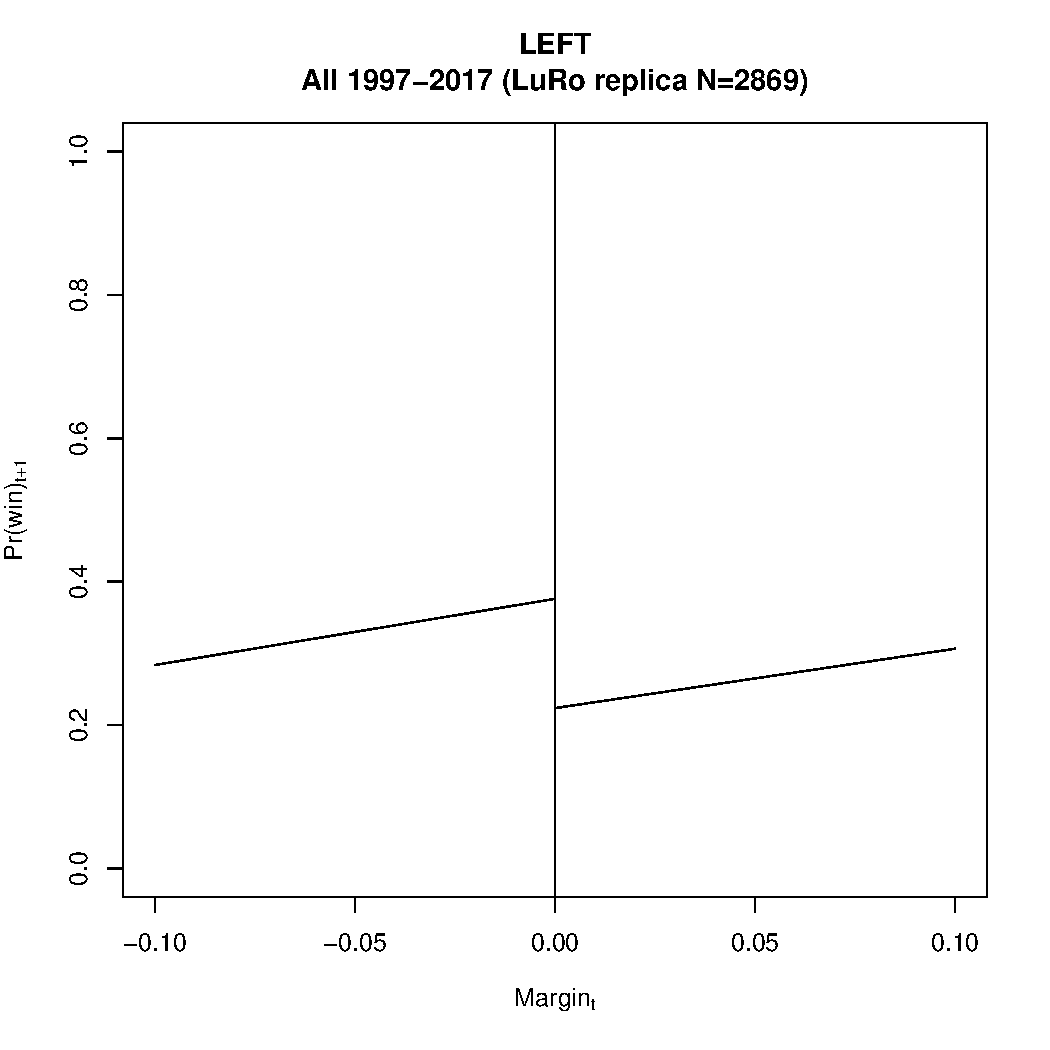
\includegraphics[width=.45\columnwidth]{../plots/leftREPLICAlpm.pdf} \\
      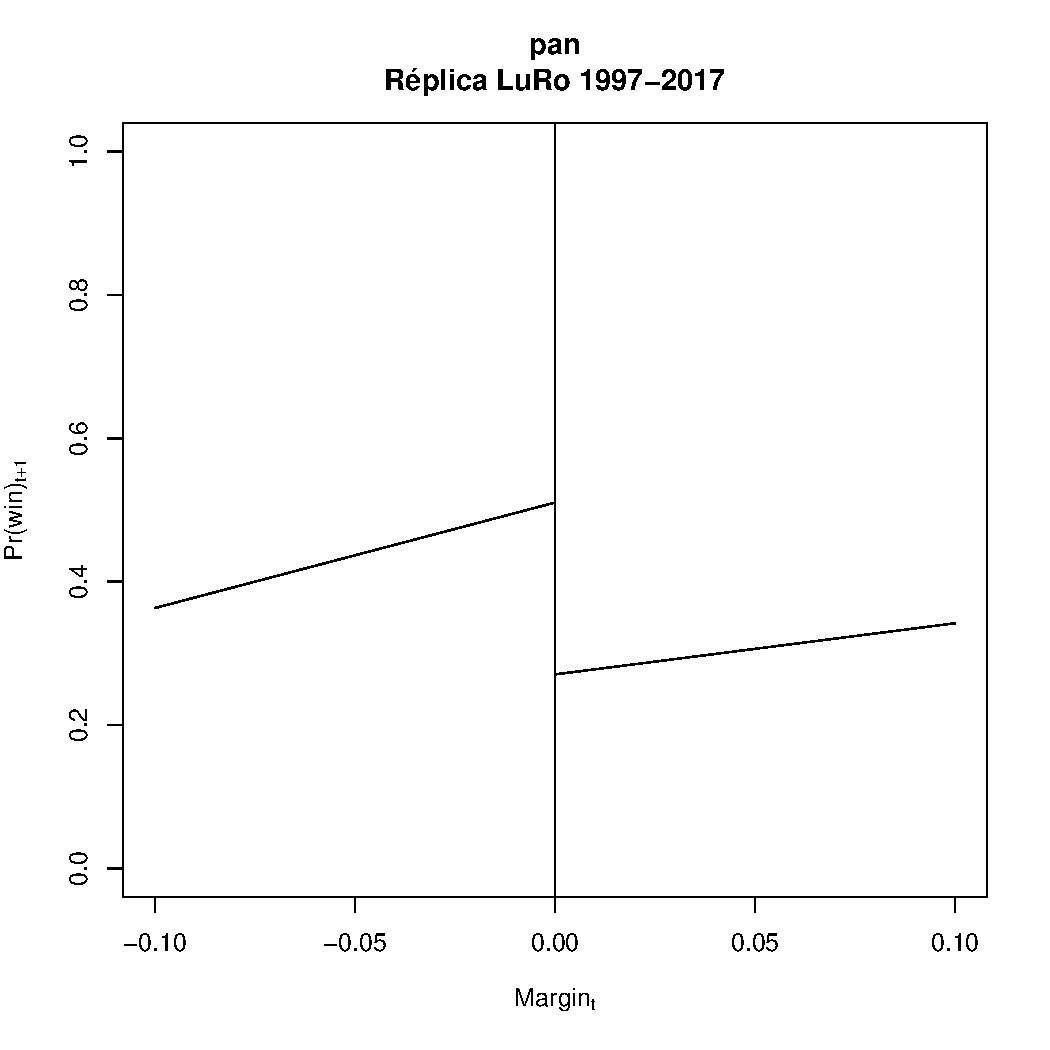
\includegraphics[width=.45\columnwidth]{../plots/panREPLICAlpm.pdf} \\
      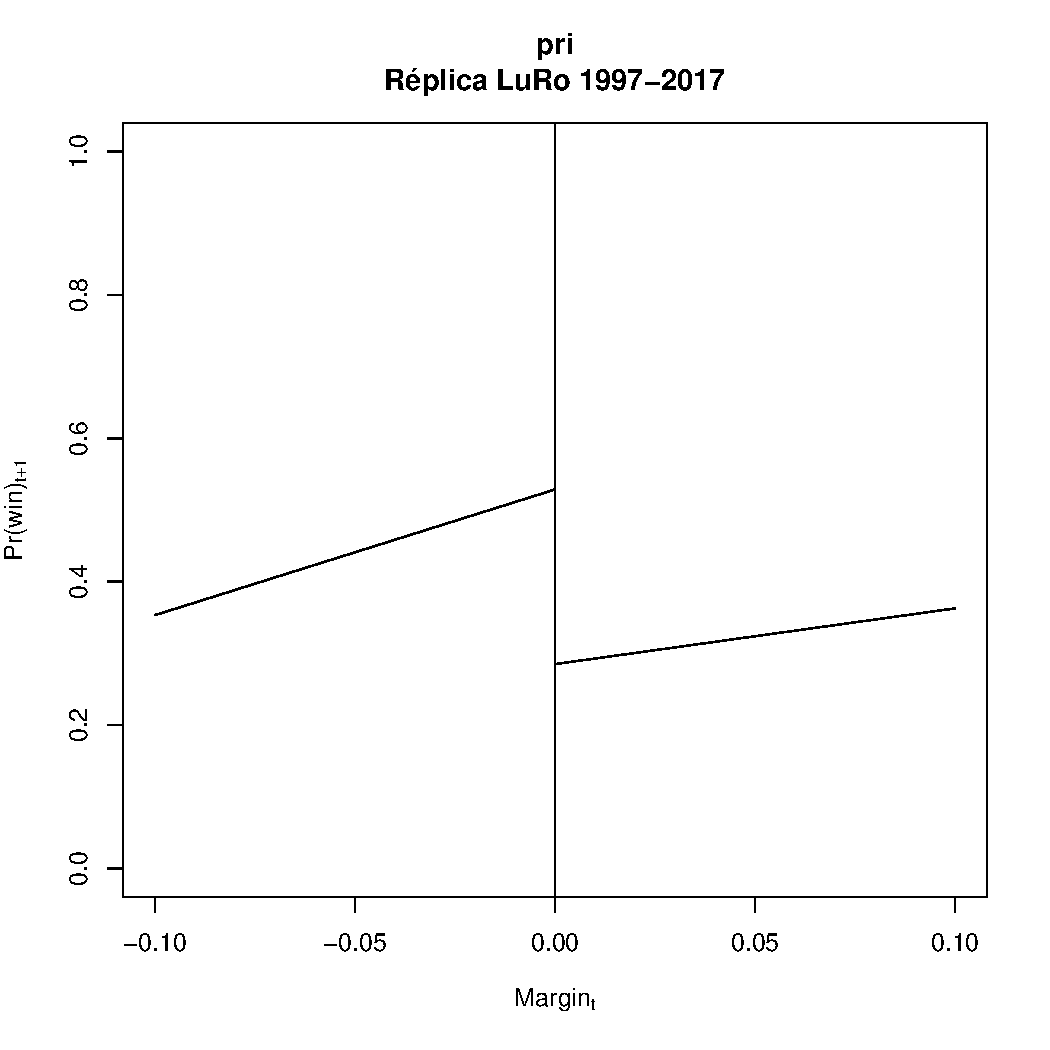
\includegraphics[width=.45\columnwidth]{../plots/priREPLICAlpm.pdf} \\
    \end{tabular}
  % }
  \caption{Modelos para el periodo 1997--2017: réplica de Lucardi--Rosas}\label{F:replica}
\end{figure}  

\singlespacing

\bibliographystyle{apsr}
%\bibliographystyle{apsrInitials}
\bibliography{/home/eric/Dropbox/mydocs/magar}

\end{document}
